\documentclass[mscthesis, 11pt, oneside, openany]{usiinfthesis}

\usepackage[utf8]{inputenc} 
\usepackage[T1]{fontenc}
\usepackage{textcomp}

\usepackage{lipsum}
\usepackage{afterpage}

\usepackage[font=scriptsize,labelfont=bf]{caption}
\usepackage{float}
\usepackage{blindtext}
\usepackage{pdfpages}

\usepackage{tocbibind} % auto add contents, tables and figures to the toc
\setcounter{tocdepth}{2}
\setcounter{secnumdepth}{6}

\usepackage{tocloft}
\setlength{\cftfignumwidth}{3em}

\usepackage{enumitem}

\usepackage{graphicx}
\pdfsuppresswarningpagegroup=1
\usepackage{caption}
%\usepackage[justification=justified,singlelinecheck=false]{caption}
\usepackage{subcaption}

\usepackage{url}
\makeatletter
\g@addto@macro{\UrlBreaks}{\UrlOrds}
\makeatother
\PassOptionsToPackage{hyphens}{url}
%Import the natbib package and sets a bibliographys and citation styles
\bibliographystyle{plainnat}
\setcitestyle{numbers,open={[},close={]}}
\renewcommand{\bibname}{References}

\newfloat{Equation}{htbp}{equ}[chapter]
\newcommand{\listequationsname}{Equations}

\usepackage{xcolor}
\usepackage{listings,lstautogobble}
\definecolor{gray}{gray}{0.5}
\colorlet{commentcolour}{green!50!black}
\colorlet{stringcolour}{red!60!black}
\colorlet{keywordcolour}{blue}
\colorlet{exceptioncolour}{yellow!50!red}
\colorlet{commandcolour}{magenta!90!black}
\colorlet{numpycolour}{blue!60!green}
\colorlet{literatecolour}{magenta!90!black}
\colorlet{promptcolour}{green!50!black}
\colorlet{specmethodcolour}{violet}
\newcommand*{\literatecolour}{\textcolor{literatecolour}}
\newcommand*{\pythonprompt}{\textcolor{promptcolour}{{>}{>}{>}}}
\lstdefinestyle{python}{
	language=python,
	showtabs=true,
	tab=,
	tabsize=4,
	basicstyle=\ttfamily\footnotesize,
	stringstyle=\color{stringcolour},
	showstringspaces=false,
	keywordstyle=\color{keywordcolour}\bfseries,
	emph={as,and,break,class,continue,def,yield,del,elif ,else,%
		except,exec,finally,for,from,global,if,in,%
		lambda,not,or,pass,print,raise,return,try,while,assert,with},
	emphstyle=\color{blue}\bfseries,
	emph={[2]True, False, None},
	emphstyle=[3]\color{commandcolour},
	morecomment=[s]{"""}{"""},
	commentstyle=\color{commentcolour}\slshape,
	emph={array, matmul, ones, transpose, float32},
	emphstyle=[4]\color{numpycolour},
	emph={[5]assert,yield},
	emphstyle=[5]\color{keywordcolour}\bfseries,
	emph={[6]range},
	emphstyle={[6]\color{keywordcolour}\bfseries},
	literate=*%
	{:}{{\literatecolour:}}{1}%
	{=}{{\literatecolour=}}{1}%
	{-}{{\literatecolour-}}{1}%
	{+}{{\literatecolour+}}{1}%
	{*}{{\literatecolour*}}{1}%
	{**}{{\literatecolour{**}}}2%
	{/}{{\literatecolour/}}{1}%
	{//}{{\literatecolour{//}}}2%
	{!}{{\literatecolour!}}{1}%
	{<}{{\literatecolour<}}{1}%
	{>}{{\literatecolour>}}{1}%
	{>>>}{\pythonprompt}{3},
	frame=trbl,
	rulecolor=\color{black!40},
	backgroundcolor=\color{gray!5},
	breakindent=.5\textwidth,
	frame=single,
	breaklines=true,
	basicstyle=\ttfamily\footnotesize,%
	keywordstyle=\color{keywordcolour},%
	emphstyle={[7]\color{keywordcolour}},%
	emphstyle=\color{exceptioncolour},%
	literate=*%
	{:}{{\literatecolour:}}{2}%
	{=}{{\literatecolour=}}{2}%
	{-}{{\literatecolour-}}{2}%
	{+}{{\literatecolour+}}{2}%
	{*}{{\literatecolour*}}2%
	{**}{{\literatecolour{**}}}3%
	{/}{{\literatecolour/}}{2}%
	{//}{{\literatecolour{//}}}{2}%
	{!}{{\literatecolour!}}{2}%
	{<}{{\literatecolour<}}{2}%
	{<=}{{\literatecolour{<=}}}3%
	{>}{{\literatecolour>}}{2}%
	{>=}{{\literatecolour{>=}}}3%
	{==}{{\literatecolour{==}}}3%
	{!=}{{\literatecolour{!=}}}3%
	{+=}{{\literatecolour{+=}}}3%
	{-=}{{\literatecolour{-=}}}3%
	{*=}{{\literatecolour{*=}}}3%
	{/=}{{\literatecolour{/=}}}3%
}
\lstnewenvironment{python}
{\lstset{style=python}}
{}

% Load the package with the acronym option
\usepackage[titletoc,page]{appendix}
\makeatletter\@openrightfalse\makeatother

\usepackage[acronym,automake,nonumberlist]{glossaries}
%\usepackage[noindex]{glossaries-extra}

% Generate the glossary
\makeglossaries
\renewcommand*\glspostdescription{\dotfill}
\renewcommand*\acronymname{ }

\newcommand{\nomNoPrint}[3]{\newglossaryentry{#1}{
		name={#2},
		symbol={#2},
		description={#3},
		sort={A\three@digits{\value{page}}}
	}\glsadd[format=hyperbf]{#1}}   
\makeatother

\newcommand{\nom}[3]{\nomNoPrint{#1}{#2}{#3}#2}

\newglossaryentry{fig}{
	name={Fig.},
	description={Figure}
}


\newglossaryentry{tab}{
	name={Tab.},
	description={Table}
}

\newglossaryentry{cm}{
	name={cm},
	description={centimetre}
}

\newglossaryentry{s}{
	name={s},
	description={seconds}
}


\newglossaryentry{h}{
	name={h},
	description={hours}
}

\newglossaryentry{cm/s}{
	name={cm/s},
	description={centimeters per second}
}

\newglossaryentry{wrt}{name={w.r.t.},description={with respect to}}

\newacronym{idsia}{IDSIA}{Istituto Dalle Molle di Studi sull’Intelligenza Artificiale}
\newacronym{faa}{FAA}{United States Federal Aviation Administration}
\newacronym{ros}{ROS}{Robot Operating System}
\newacronym{vr}{VR}{Virtual Reality}
\newacronym{ar}{AR}{Augmented Reality}

\newacronym{fps}{FPS}{frames per second}
\newacronym{mp}{MP}{megapixel}
\newacronym{fov}{FOV}{field of view}
\newacronym{mocap}{MoCap}{motion capture}
\newacronym{dof}{DoF}{degrees of freedom}
\newacronym{ir}{IR}{infrared}

\newacronym{wrt}{wrt}{with respect to}

\newacronym{ai}{AI}{Artificial Intelligence}
\newacronym{xai}{XAI}{Explainable AI}
\newacronym{ml}{ML}{Machine Learning}
\newacronym{dl}{DL}{Deep Learning}

\newacronym{nn}{NN}{Neural Network}
\newacronym{dnn}{DNN}{Deep Neural Network}
\newacronym{ann}{ANN}{Artificial Neural Network}
\newacronym{rnn}{RNN}{Recurrent Neural Network}
\newacronym{rl}{RL}{Reinforcement Learning}
\newacronym{cnn}{CNN}{Convolutional Neural Network}
\newacronym{resnet}{ResNet}{Residual Neural Network}

\newacronym{cam}{CAM}{Class Activation Mapping}
\newacronym{gradcam}{Grad-CAM}{Gradient-weighted Class Activation Mapping}
\newacronym{gmm}{GMM}{Gaussian Mixture Model}

\newacronym{gt}{GT}{ground truth}
\newacronym{adam}{ADAM}{Adaptive Moment Estimation}
\newacronym{mae}{MAE}{Mean Absolute Error}
\newacronym{mse}{MSE}{Mean Squared Error}
\newacronym{rmse}{RMSE}{Rooted Mean Squared Error}
\newacronym{r2}{R$^2$}{R Squared}

\newcommand{\footlabel}[2]{%
	\addtocounter{footnote}{1}%
	\footnotetext[\thefootnote]{%
		\addtocounter{footnote}{-1}%
		\refstepcounter{footnote}\label{#1}%
		#2%
	}%
	$^{\ref{#1}}$%
}

\newcommand{\footref}[1]{%
	$^{\ref{#1}}$%
}

\lstdefinelanguage{algebra}
{morekeywords={import,sort,constructors,observers,transformers,axioms,if,
else,end},
sensitive=false,
morecomment=[l]{//s},
}


%%%%%%%%%%%%%%%%%%%%%%%%%%%%%%%%%%%%%%%%%%%%%%%%%%%%%%%%%%%%%%%%%%%%%%%%%%%%%%%%%%%%%%%%%%%%%%%%%%%%%%%%%%%%%%


\title{Interpretation of Neural Networks and \\ Advanced Image Augmentation for Visual Control of Drones in Human Proximity} %compulsory
%\specialization{Dependable Distributed Systems}%optional
%\subtitle{Subtitle: Reinventing the World} %optional 

\author{Marco Ferri} %compulsory
\begin{committee}
\advisor{Dr.}{Alessandro}{Giusti} %compulsory
\coadvisor{PhD Stud.}{Dario}{Mantegazza}{} %optional
\end{committee}

\Day{22} %compulsory
\Month{February} %compulsory
\Year{2021} %compulsory, put only the year
\place{Lugano} %compulsory

\dedication{To my mother and father} %optional
\openepigraph{``Sometimes it is the people no one can imagine anything of, who do the things no one can imagine.''}{The Imitation Game} %optional


%\makeindex %optional, also comment out \theindex at the end


%%%%%%%%%%%%%%%%%%%%%%%%%%%%%%%%%%%%%%%%%%%%%%%%%%%%%%%%%%%%%%%%%%%%%%%%%%%%%%%%%%%%%%%%%%%%%%%%%%%%%%%%%%%%%%

\begin{document}


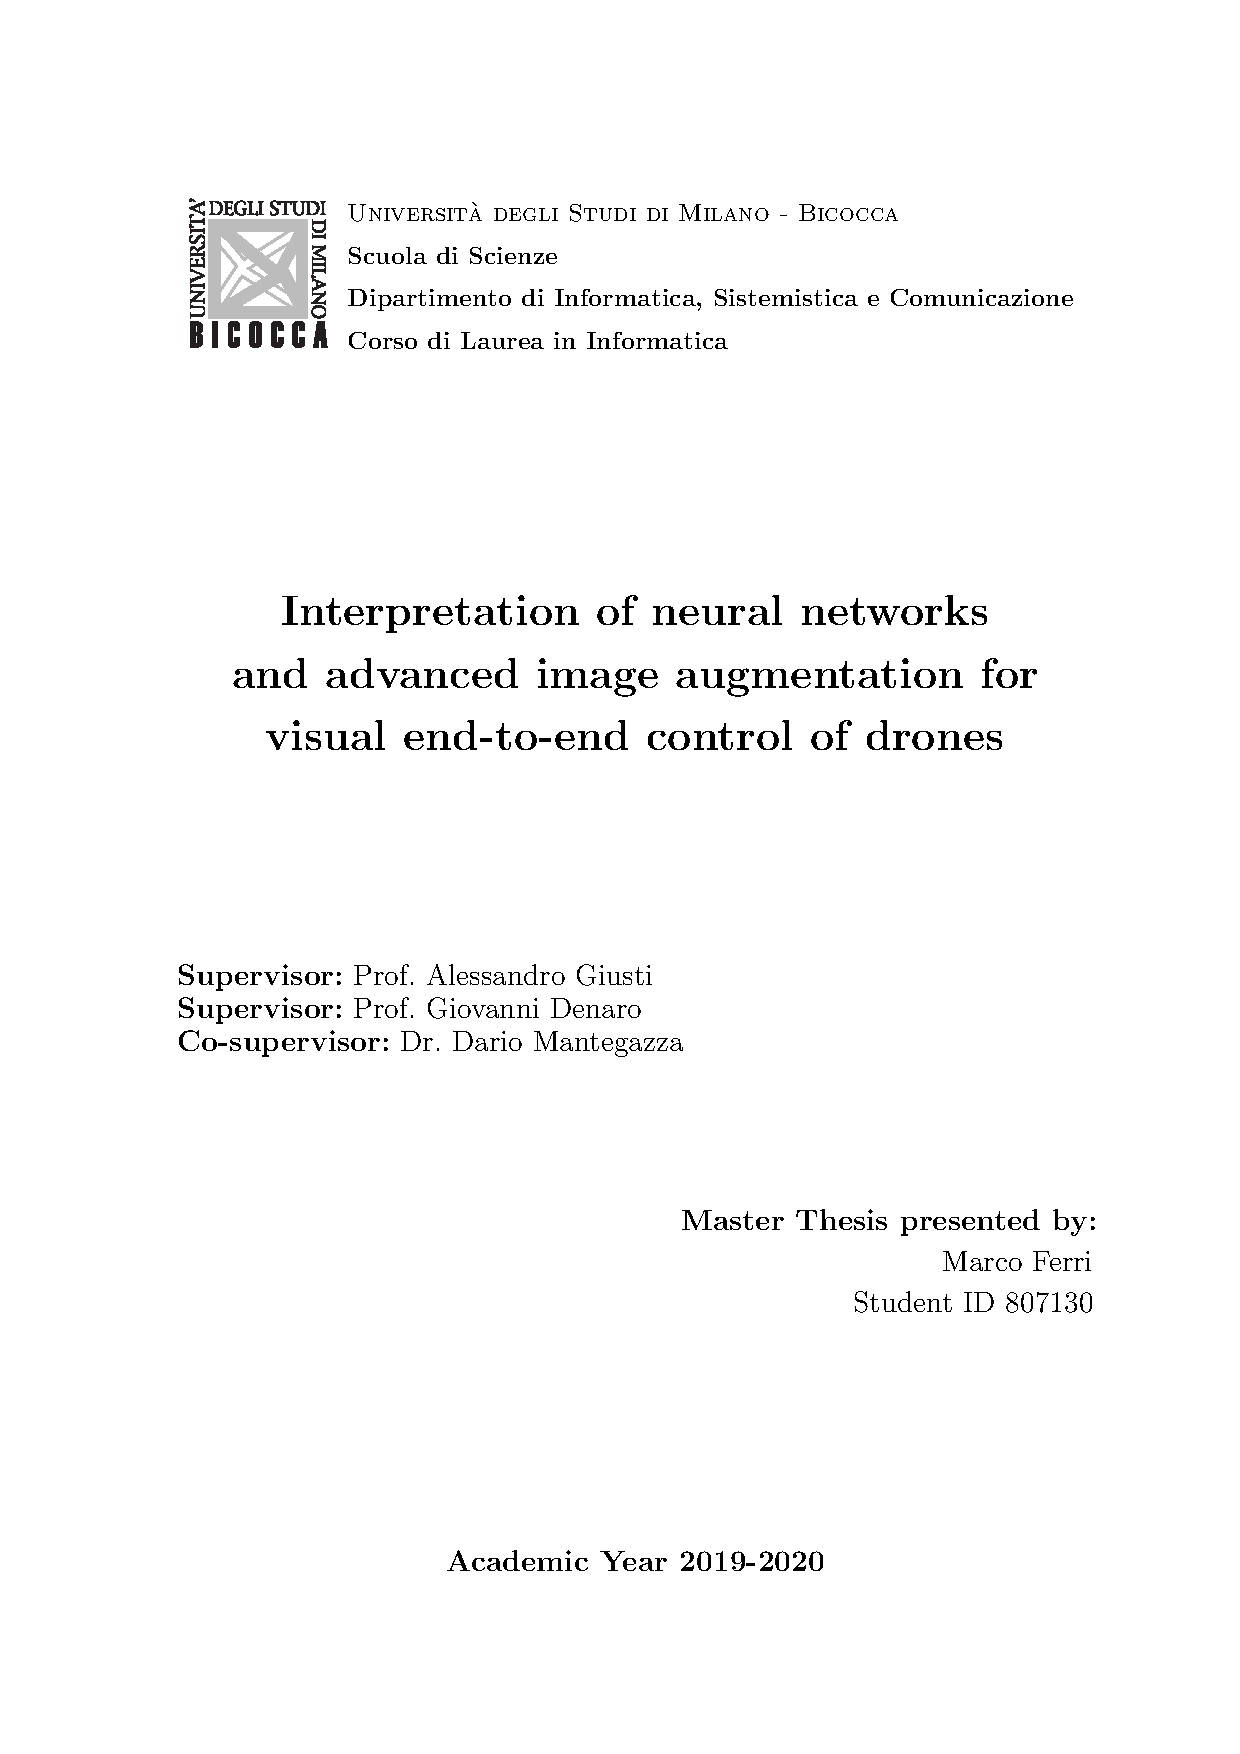
\includepdf{contents/images/frontespizio-unimib}
% \maketitle %generates the titlepage, this is FIXED
\let\cleardoublepage\clearpage




\frontmatter %generates the frontmatter, this is FIXED
%\let\cleardoublepage\clearpage



\begingroup
%\let\cleardoublepage\clearpage

\begin{abstract}
\addcontentsline{toc}{chapter}{Abstract}  % added 

%We consider the task of predicting the pose of a person moving in front of a drone, using the input images coming from an on-board camera. We aim to improve the generalization capabilities of a machine learning model designed for this intent.

We consider the task of predicting the pose of a person moving in front of a drone, using the input images coming from an on-board camera. We aim to improve a machine learning model designed for this intent \cite{mantegazza2019visionbased}. The approach relies on supervised learning to perform a regression on the user's pose through a Residual Neural Network. The training data is collected in a dedicated drone arena, using a Motion Capture system to acquire the ground truth. The prototype achieves good performance inside the arena but cannot fulfill its duty in unknown environments.

First, we understand the main issues of the learned task through network interpretation. Applying Grad-CAM, we observe that the model not only focus on the user who is actually facing the drone’s camera. Instead, various portions of the input images are considered when the model makes its predictions. We assume that the neural network has undesirably learned some details about the drone arena in which the dataset has been collected.

As a solution, we develop an advanced data augmentation technique designed for
%enhanching the generalization capabilities of the model, by
breaking the relationship between the model's learning and the training room. Our approach makes use of Mask R-CNN for computing the user's mask from each sample in the original training set. Then, we use the computed masks for replacing the corresponding images' background and retraining the neural network.

We run experiments that show that our proposal is successful both from quantitative and qualitative viewpoints. The model, trained on the augmented dataset, produces satisfactory results in a large variety of real-world scenarios.
\end{abstract}

\begin{acknowledgements}
\addcontentsline{toc}{chapter}{Acknowledgements}  % added 

My most grateful thanks go to my supervisors Alessandro and Dario for having thoroughly assisted me, both technically and emotionally, during the entire development of this thesis.

\smallskip

Thanks to the University of Milano-Bicocca for the opportunity of participating in this amazing Double Degree Program and to USI Università della Svizzera Italiana for immediately making me feel at home. Thanks to all my classmates and friends, who have lightened my journey over all these years.

\bigskip

A special thanks to my lovely Nadia, for always being by my side, supporting me unconditionally, and making me laugh with every single breath.

\smallskip

Un ultimo e sentito grazie ai miei genitori, per aver sempre appoggiato le mie scelte e per avermi trasmesso i loro valori, rendendomi la persona che sono oggi.
\end{acknowledgements}

\endgroup


\clearpage

%\pdfbookmark{\contentsname}{Contents}
\tableofcontents 
\newpage

\begingroup
\let\cleardoublepage\clearpage
\listoffigures %optional
% \addcontentsline{toc}{chapter}{List of Figures}
 
\listoftables %optional
% \addcontentsline{toc}{chapter}{List of Tables}

%%\cleardoublepage
%\listof{Equation}{\listequationsname}
%\addcontentsline{toc}{chapter}{List of \listequationsname}

%\lstlistoflistings
%\addcontentsline{toc}{chapter}{List of Listings}
%\endgroup
%%\let\cleardoublepage\relax

\makeatletter
\renewcommand\mainmatter{\clearpage\@mainmattertrue\pagenumbering{arabic}}
\makeatother

%%%%%%%%%%%%%%%%%%%%%%%%%%%%%%%%%%%%%%%%%%%

\mainmatter

\begingroup
\let\cleardoublepage\clearpage
\chapter{Introduction}
%\addcontentsline{toc}{chapter}{Introduction}
%\markboth{}{}
\label{chap:intro}

\glsresetall

Nowadays, the use of \gls{ai} is increasing in Robotics and Computer Vision. Research in the area aims to find innovative solutions, especially using \gls{dl}, for well-known yet complex goals such as autonomous navigation, human-robot interaction, and object detection. A trending approach in the last years is Imitation Learning \cite{imitation_learning_survey}. It consists of training a \gls{nn} on a given task by observing the behavior of experienced agents in the same job.

Being a branch of \gls{dl}, also \gls{il} requires a large amount of data to train on. A fundamental aspect in research is the collection of real-world data to build datasets for \gls{ml} applications. However, in many cases, data is not easy to retrieve. In Robotics, datasets acquired with physical robots are usually limited in size or do not provide a faithful representation of the real world. This happens because many Robotics applications require the robots to act in a well-controlled environment, due to physical, technical, or legal constraints. This is why, in order to provide enough training data to the \gls{ml} model, Imitation Learning often relies on datasets generated in simulation. If the simulator is good enough in proposing the neural network a good variety of realistic data, then the real world may appear to the model as just another variation of the training environment.  The technique is known as Domain Randomization \cite{tobin2017domain}, designed to transfer a learned task from one domain to another.

\medskip

In this thesis, we consider an Imitation Learning technique for teaching a drone how to continuously hover in front of a moving person. We focus on the existing work from Mantegazza et al. \cite{mantegazza2019visionbased}, aiming to improve the generalization capabilities of the model. In the paper, the authors propose a reactive control procedure for controlling the quadcopter using the \gls{ml}-inferred user's pose. They build a \gls{resnet} to predict the user's 3D coordinates with respect to the drone, using in input the images coming from an on-board camera. The network is modeled to perform regression through supervised learning, in which the ground truth is given by an external \gls{mocap} system.

The original approach is an interesting starting point for many other Robotics applications, as it provides a small but fast neural network capable of producing real-time inferences. Also, it explores a challenging task in the research area of human-drone interaction, which will most probably experience interesting growth in the next years \cite{human-drone-sota}. The main issue of the proposed model is the inability of making proper predictions outside of the training room. Since the data collection requires a dedicated \gls{mocap} system to acquire the ground truth, the possibility of recording new data in different locations must be excluded. A related work \cite{zimmerman2020thesis} explored different kinds of data augmentation for the task, applying classical image transformations. Results are encouraging but still not enough to make the model able to generalize the task in unknown environments.

\medskip

Our goal is to understand the underlying causes of the issue and find a solution to the generalization problem. First, we apply \gls{gradcam} \cite{Selvaraju_2019} for network interpretation. In a few words, the algorithm produces a heatmap on the given images which enables the visualization of the input regions actually responsible for predicting a certain model’s output. Using \gls{gradcam}, we discover that the frontal drone model is not only considering the people in the input images for producing its outputs. Instead, many recurrent elements in the training set are attracting the network's attention. We want to reduce the model overfitting by eliminating the biases coming from the data. 

As a solution, we propose an innovative pipeline for image augmentation, inspired by Domain Randomization \cite{weng2019DR}. Our approach consists of modifying the original dataset through the replacement of the camera's frames' background. We rely on Mask R-CNN \cite{he2018mask}, a state of the art deep learning algorithm for object detection and segmentation. We adopt the algorithm to pre-compute the users' masks, used during training to blend the input frames with other images, serving as the backgrounds. For the replacement, we use images from a public dataset for Indoor Scene Recognition \cite{cvpr09}. The technique allows the simulation of various scenarios without the need to actually collecting new data. We also apply classic image augmentation before retraining the \gls{resnet} architecture on the background-replaced dataset. Several quantitative and qualitative experiments demonstrate the robustness of the solution, providing satisfactory results in a large variety of real-world scenarios, both indoor and outdoor.

\medskip

The solution we propose is reasonably applicable to other Computer Vision tasks. In particular, the usage of a computationally expensive method such as Mask R-CNN for pre-processing data enables a severe expansion of a given dataset. Hence, the augmented dataset can be used to train lighter models, which may require human or object recognition capabilities at a cheaper cost.

\clearpage

This work is the result of a collaboration with the Robotics research team at \gls{idsia}, in Lugano (Switzerland). The thesis has been submitted to the \gls{unimib} and \gls{usi} in the context of a Double Degree Program for the Master of Science in Informatics.

The entire source code and any additional resources, presentations, or videos are publicly available at \url{https://github.com/mferri17/cnn-drone-befree}.




\section*{Thesis Outline}
\label{sec:outline}

The document is composed of seven chapters, briefly described here:

\begin{itemize}
	\item This chapter provides an overview of our work and its structure.
	\item Chapter \ref{chap:theory} gives a theoretical introduction on the concepts used in the thesis and explores the main literature related with the thesis.
	\item Chapter \ref{chap:system} illustrates the composition of the existing system and lists the main frameworks used during the development of our software.
	\item Chapter \ref{chap:design} summarizes our design process and choices by presenting the experiments conducted for shaping our final solution.
	\item Chapter \ref{chap:implementation} carefully describes practical details of our implementation from both methodology and technical perspectives.
	\item Chapter \ref{chap:evaluation} shows the evaluation results for assessing our approach validity and robustness from a quantitative and a qualitative point of view.
	\item Chapter \ref{chap:conclusion} concludes the thesis, summarizing what has been done with some final thoughts and future works.
\end{itemize}

Appendix \ref{chap:extra-figures} also contains additional images, not inserted in the main chapters, that add minor interesting details on various topics.






\chapter{Theoretical Foundation}
\label{chap:theory}

%\lipsum[1]



\section{Robotics}
\label{sec:robotics}

%\subsection{Pose}
%\label{subsec:robot-pose}
%
%\subsection{Control Theory}
%\label{subsec:robot-control}




\section{Machine Learning}
\label{sec:machine-learning}

%\subsection{Supervised Learning}
%\label{subsec:supervised-learning}
%
%\subsection{Convolutional Neural Networks}
%\label{subsec:cnn}
%
%\subsection{Residual Neural Networks}
%\label{subsec:resnet}




\section{Human-drone Interaction}
\label{sec:human-drone-interaction}

A good variety of research can be found on human-robot interaction and a lot is yet to come. In the field, drones represent a specific segment due to their ability to freely move in the 3D space, opening access to new use cases while representing a real challenge for professionals and researchers.

In this section, we firstly present a general overview on the topic, then we focus on related work by \gls{idsia}.



\subsection{The State of the Art of Human–Drone Interaction}
\label{subsec:human-drone-sota}

A recent article, published in Nov 2019 for IEEE Access (\cite{human-drone-sota}), explores literature and state of the art for human-drone interaction. Drones range from small toy-grade remote-controlled aircraft to fully-autonomous systems capable of decision-making through a large variety of sensors. Their usage grew a lot in the last years and it is expected to keep growing, thanks to decreasing costs and powerful features they can provide both for personal, commercial, and social usage.

\gls{faa} expects that total drone registrations will increase by more than 60\% between 2018 and 2022 with a particular increment in the commercial sector rather than the hobbyist one, even though the latter still counts the largest number of units. Moreover, \gls{faa} reports that almost half of drones usage is for aerial photography (48\%), followed by industrial inspection (28\%) and agriculture (17\%). Accordingly to \cite{human-drone-sota}, drones will become ubiquitous to society and, in the next decade, they will be extensively used in advertising, shipping, sports, emergency, and many other fields for augmenting human capabilities.

The main concerns about drones today regard safety issues caused by propellers and limited flight times, usually no longer than 30 minutes due to limited battery capacity. Research in the sector of human-drone interaction mainly focuses on their control (through gestures, voice, or custom interfaces), communication between the user and the drone itself (in terms of acknowledgment and intents), perception of users' safety during flight, and innovative use cases. 



\subsection{Vision-based Control of a Quadrotor in User Proximity}
\label{subsec:sota-dario}

Our work is built upon the original master thesis (\cite{mantegazza2018thesis}) and paper (\cite{mantegazza2019visionbased}) \textit{Vision-based Control of a Quadrotor in User Proximity: Mediated vs End-to-End Learning Approaches} from Dario Mantegazza, developed at \gls{idsia} in Lugano. In his thesis, the author proposes a machine learning model for teaching a drone to interact with a person by continuously flying to face the user frontally, towards the direction of the head. The problem is approached as a reactive control procedure and addressed with supervised learning, thus provides an interesting starting point for many other robotics applications. 

The author collects data and tests his model on the Parrot Bebop 2, a 500grams drone commonly used for photography and leisure purposes, capable of effective video stabilization. However, the software runs off-board, on a dedicated computer remotely connected through WiFi. 

A considerable amount of flights is recorded for building the training data by programmatically flying the drone in front of a person, controlling it through an omniscient controller that knows both the drone's and user's pose. Images produced by the front-facing camera of the drone are used as input for a custom-designed \gls{resnet} architecture to infer the relative user's position \gls{wrt} the drone. Practically, the neural network performs a regression on the four variables that form the user's pose (X, Y, Z, YAW) and learns to predict their values by using spacial information contained in the input images. 

In the paper, the author also makes a comparison between the mediated approach described above and another end-to-end approach that directly learns control signals\footnote{desired pitch, roll, yaw, and vertical velocity} for the drone, instead of the user's pose. Another experiment also considers a learned controller. All the solutions provide similar results, but the former can be adapted to other tasks by simply designing a custom controller, providing a more transparent and analyzable solution\footnote{take a look at image \ref{fig:proximitynet-architecture-paper3approaches} for details about models architectures designed for the three approaches}.

Even though this kind of problems on human recognition and pose estimation could be faced with more advanced deep learning algorithms, making a simple regression on four variables allows the network to be fairly small, so that the prediction task is light, fast to execute, and possibly portable on low-end devices.

\medskip

Network and dataset defined in \cite{mantegazza2019visionbased} have been used for our entire project, so the original code repository\footnote{\url{https://github.com/idsia-robotics/proximity-quadrotor-learning}} is available for reference. The next chapters constantly make use of this particular model architecture, which will be further explained in section \ref{sec:proximitynet}. 

Having no official name, for enhancing readability, the custom \gls{resnet} architecture proposed by the author will be simply called \textit{ProximityNet}. For a better understanding, also a good descriptive video is available at \url{https://drive.switch.ch/index.php/s/MlEDrsuHcSl5Aw5}.



\subsection{Embedded Implementation of Controller for Nano-Drones}
\label{subsec:sota-nicky}

Autonomous navigation is an important and well-known area of research in robotics, which usually requires accomplishing complex and computationally-expensive tasks such as localization, mapping and path planning. Recent studies have started to approach autonomous driving through deep learning and imitation learning\cite{imitation-learning}, where neural networks learn by imitating human behavior in specific tasks. 

\medskip

In 2018, researchers at the UZH University of Zürich have demonstrated that \gls{resnet}s are able to provide satisfactory performance in the field (\cite{Loquercio_2018}). They developed DroNet, a forked \gls{cnn} that predicts, from a single gray-scale image, a steering angle and a collision probability. In other words, the model learns to steer and avoid obstacles from forward-looking videos recorded by cars and bikes while driving in real contexts. In this case, both the prediction and controller tasks were powered off-drone on a dedicated computer, remotely connected through WiFi. 

A year later, ETH Zürich was able to develop PULP-DroNet, porting the \gls{cnn} on the Crazyflie\footnote{\url{https://www.bitcraze.io/products/crazyflie-2-1/}}, a nano-drone with a size of only 3 $3 \times 3$ centimeters for a weight of 27 grams. They propose a general methodology for deploying on-board deep learning algorithms for ultra-low-power devices \cite{palossi2019pulpdronetIoTJ}, without any need for an external laptop to run the software.

\medskip

Inspired by PULP-DroNet, \gls{idsia} adapted its ProximityNet to work on-board the Crazyflie with excellent results \cite{zimmerman2020thesis}. The nano-drone is able to achieve good quantitative and qualitative performance, regardless of any problem deriving from working with such low-end devices. The main challenges are represented by low computational power, energy consumption management, and low-fidelity camera with no video stabilization\footnote{Himax HM01B0 camera, able to produce $320 \times 320$ \gls{mp} at 60 FPS. However, the frame rate is incredibly reduced during data collection due to platform limitation for image transfer.}.




\section{Network Interpretability}
\label{sec:network-interpretability}

\glsreset{ml}
\glsreset{nn}

Deep \gls{nn}s learn abstract representations for finding a logical mapping between their input and output, determined by well-defined mathematical computations that involve the input itself and the progressively learned network parameters. Inspired by biological brains, this approach seems to be incredibly effective on a huge variety of tasks.

Unlike other \gls{ml} techniques, \gls{nn} are known to produce "black-box" models, particularly hard to understand even from domain experts. Their reasoning and comprehension are intrinsic in the network parameters, which are nothing but numbers.

\medskip 

However, when working with real-world problems, it is extremely important to be able to explain what a \gls{ml} model is actually understanding. This is crucial for building trust in algorithms and to be sure there are no undesirable biases in the models, which could raise serious problems especially in critical fields such as medicine and law.

\gls{xai} is the field of study which tries to make \gls{ml} results, and their underlying basis for decision-making, properly understandable to humans (\cite{xai-wiki}). 

\medskip 

Regarding \gls{xai} for \gls{cnn}s, researchers have developed many techniques for understanding what a \gls{nn}s actually care of when producing an output based on an input image. Main efforts regard feature visualization and attribution, but recent advanced studies have also shown how these methods can be used altogether (\cite{olah2018the}).

This section briefly explains these two major areas for \gls{cnn} interpretability, with a particular focus on spatial attribution, the chosen methodology for our work.



\subsection{Feature Visualization}

Sources: \cite{olah2017feature}



\subsection{Spatial Attribution with GradCAM}
\label{subsec:gradcam-theory}

Sources: \cite{Selvaraju_2019}, \cite{gradcam_medium}

\begin{figure}[!htb]
	\centering
	\includegraphics[width=0.9\textwidth]{"contents/images/gradcam/02-gradcam-schema"}
	\caption[\gls{gradcam} schematic functioning]{\gls{gradcam} schematic functioning (\cite{Selvaraju_2019})}
	\label{fig:gradcam-schema}
\end{figure}

\begin{figure}[!htb]
\centering
\includegraphics[width=0.9\textwidth]{"contents/images/gradcam/02-gradcam-catdog"}
\caption[\gls{gradcam} example on dog-cat classification]{\gls{gradcam} example on dog-cat classification (\cite{Selvaraju_2019})}
\label{fig:gradcam-catdog}
\end{figure}




\section{Network Generalization}
\label{sec:network-generalization}



\subsection{Data Augmentation}
\label{subsec:data-augmentation}



\subsection{Domain Randomization}
\label{subsec:domain-randomization}

\textbf{TODO}

Summary from \cite{mehta2019active}

See \cite{weng2019DR_explanation}
 
"Domain randomization is a popular technique for improving domain transfer, often used in a zero-shot setting when the target domain is unknown or cannot easily be used for training. In this work, we empirically examine the effects of domain randomization on agent generalization. Our experiments show that domain randomization may lead to suboptimal, high-variance policies, which we attribute to the uniform sampling of environment parameters."


\subsubsection{Virtual Simulation}
\label{subsec:virtual-simulation}

Imitation learning through simulation is recently becoming an interesting and successful approach for both reinforcement learning (\cite{imitation_learning_survey} and \cite{imitation_learning_3d_navigation}) object recognition (\cite{tobin2017domain}, \cite{weng2019DR}).

Robot and environment can be replicated through a dedicated simulator such as Gazebo\footnote{\url{http://gazebosim.org/}}, often used in robotics with \gls{ros}\footnote{\url{https://www.ros.org/}} due to its straightforward integration, or even with general-purpose graphic engines. Unreal Engine\footnote{\url{https://www.unrealengine.com/en-US/}} Unity\footnote{\url{https://unity.com/}} are well-known simulators designed for game-development, but recently used for \gls{vr} and \gls{ar} applications. They give developers unlimited possibilities, carefully supported by solid physics engines and active communities.

\medskip

Given the difficulty of collecting data for our task, exploring the possibility of simulating the entire scenario in a 3D virtual-world is intriguing, especially to replace the need for a complex \gls{mocap} system. Integrating odometry support, drone and people can be thoroughly modeled to act as in the real world, with similar movements and sensing capabilities, in order to collect the data very efficiently. The virtual simulation gives both the opportunity of reproducing real indoor/outdoor scenes, but also randomizing the background with artificially generated textures.

Even though the approach appears to obtain sub-optimal results, a complete and adaptable implementation requires a lot of effort, yet unlocking a huge number of possibilities. Considering the consistent amount of fine details to consider and issues that can arise during the development of such simulators, we opt instead to work with an easier generalization pipeline, that mostly concerns machine learning only.


\subsubsection{Background Replacement with Mask R-CNN}
\label{subsec:sota-maskrcnn}

\textbf{TODO}

Previous works on images: \cite{yue2019domain}, \cite{Takahashi_2020}

MaskRCNN: \cite{he2018mask}, \cite{maskrcnn_explanation}, \cite{maskrcnn_arcgis}




\chapter{System Description}
\label{chap:system}

\glsresetall

We focus on improving the original work from Mantegazza et al. \cite{mantegazza2019visionbased}, introduced in section \ref{subsec:sota-dario}. This chapter aims to provide a generic view of the system, starting from its main components and how they interact for flying and controlling the drone. Then, we present tools, libraries, and dataset we are working with to enhance the model generalization capabilities.




\section{Environment}
\label{sec:hardware}

Working from a machine learning perspective, our task does not require interaction with physical components. However, it is helpful to know the environment in which the drone was originally taught to fly. This is physically located in Manno (Switzerland) at \gls{idsia}\footnote{now relocated to Lugano}.



\subsection{Parrot Bebop Drone 2}
\label{subsec:bebop}

\begin{figure}[!htb]
	\centering
	\includegraphics[width=.8\textwidth]{"contents/images/03-Parrot-Bebop-2"}
	\caption[Parrot Bebop Drone 2]{Parrot Bebop Drone 2}
	\label{fig:bebop}
\end{figure}

The entire work is built around the Parrot Bebop 2 \cite{bebop} (figure \ref{fig:bebop}), a lightweight drone (500 grams) with a size of $382 \times 328 \times 89$ millimeters. A 2700 mAh swappable battery gives power to four brushless motors and a dual-core processor with a quad-core GPU, for a maximum flight time of 25 minutes. Connectivity is provided through 2.4 GHz 802.11a/b/n/ac WiFi that enables remote control via mobile app or Parrot Skycontroller (up to a distance of 2km).

The drone is equipped with many simultaneous sensors to compute velocities, orientation, altitude, and GPS coordinates to ensure maximum stability during the whole flight. For this project, we mainly focus on its camera, which can shoot 14 \gls{mp} photos and record Full HD 1080p videos at 30 \gls{fps}. Even though the original \gls{fov} is 180°, raw camera images pass through a software stabilization that produces 16:9 images with a horizontal \gls{fov} of about 80°. Parrot's 3-axis digital stabilization technique is able to compensate for the drone's pitch and roll to provide correct-oriented horizontal images and stable videos regardless of the drone's movements.



\subsection{OptiTrack}
\label{subsec:optitrack}

To monitor the drone and the user's movement, we require a \gls{mocap} system to record 3D coordinates of objects and people in space. The technique is widely used for motion tracking in various fields such as film making and animation, virtual reality, sport, medicine, and even the military. A common way to implement a \gls{mocap} systems is by using special cameras placed around the area to be tracked. These can collect optical signals from passive\footnote{a passive marker reflect light} or active markers\footnote{an active marker emits its own light} inside the area.

\medskip

\gls{idsia} adopt OptiTrack \cite{optitrack}, which is producing real-time \gls{mocap} systems since 1996 and are today world’s choice for low-latency and high-precision 6 \gls{dof} tracking for ground and aerial robotics, both indoor and outdoor.



\subsection{Drone Arena}
\label{subsec:drone-arena}

At \gls{idsia}, a dedicated room has been equipped with a \gls{mocap} system composed of 12 OptiTrack Prime$^x$13 \gls{ir} cameras\footnote{1.3 \gls{mp}, 240 \gls{fps}, $\pm0.20$ mm 3D accuracy in a $9 \times 9$ meters area with 14mm markers} for medium-sized areas (figure \ref{fig:optitrack-camera}). They track passive markers' movements, placed both on the person's head facing the drone and on the drone itself. Schematic and actual representation of the arena are shown in figures \ref{fig:optitrack-schema} and \ref{fig:drone-arena}. Such composition can track a theoretical number of 18 drones inside an available area of $6 \times 6$ meters (here surrounded by a safety net). A virtual fence of $4.8 \times 4.8$ meters virtually constraints the total area in which the drone is allowed to fly.

\begin{figure}[!htb]
	\centering
	\includegraphics[width=1\textwidth]{"contents/images/03-optitrack-schema"}
	\caption[Schematic OptiTrack system with 12 OptiTrack Prime cameras]{Schematic OptiTrack system with 12 OptiTrack Prime cameras}
	\label{fig:optitrack-schema}
\end{figure}

\begin{figure}[!htb]
	\begin{center}
		\begin{subfigure}[h]{0.29\textwidth}
			\centering
			\includegraphics[width=1\textwidth]{"contents/images/03-optitrack-camera"}
			\caption[]{Prime$^x$13 camera}
			\label{fig:optitrack-camera}
		\end{subfigure}
		\hfill
		\begin{subfigure}[h]{0.69\textwidth}
			\centering
			\includegraphics[width=1\textwidth]{"contents/images/03-arena"}
			\caption[]{Drone with passive markers \cite{mantegazza2018thesis}}
			\label{fig:drone-arena}
		\end{subfigure}
	\end{center}
	\vspace{-0.5cm}
	\caption[Drone arena at \gls{idsia}]{Drone arena at \gls{idsia}}
\end{figure}



\section{Dataset}
\label{sec:dataset}

This section refers to the dataset defined in Mantegazza et al. \cite{mantegazza2019visionbased}, which is also used for our research.


\subsection{Collection}
\label{subsec:control}

Data have been entirely collected in the dedicated drone arena, presented in section \ref{subsec:drone-arena}. A good dataset should ideally provide images from various scenarios, but such a kind of data is not easy to record. The ground truth must be acquired by a complex and expensive \gls{mocap} system, particularly difficult to be moved and reassembled outdoor.

\medskip

The drone is controlled by a \gls{ros} script, running on a dedicated computer remotely connected through WiFi. It relies on the known user's pose - from now on, the \textit{target pose} (i.e., the pose of the user seen by the drone reference frame) - to compute acceleration commands for the drone. The script is responsible for making the drone hovering in front of the person, facing the head orientation at a predefined 1.5 meters distance.

During data collection, both user's and drone's poses are captured by the OptiTrack using proper markers placed on the drone and the person's head (picture \ref{fig:drone-facing}). The target poses over time\footnote{mathematically computed by a script from \cite{mantegazza2018thesis}}, are synchronized with the video stream coming from the camera and saved into \texttt{rosbag} files. Figure \ref{fig:drone-demo-2} shows an illustration of the system from a bird-eye view.

\begin{figure}[!h]
	\centering
	\includegraphics[width=0.5\textwidth]{"contents/images/03-drone-facing"}
	\caption[Markers placed on top of drone and user's head]{Markers placed on top of drone and user's head \cite{mantegazza2018thesis}}
	\label{fig:drone-facing}
\end{figure}

\begin{figure}[!htb]
	\centering
	\includegraphics[width=1\textwidth]{"contents/images/03-arena-demo-2"}
	\caption[OptiTrack and data collection illustration]{OptiTrack and data collection illustration \cite{mantegazza2018thesis}}
	\label{fig:drone-demo-2}
\end{figure}



\subsection{Composition}
\label{subsec:dataset-composition}

Data collected inside the arena have been used to build the dataset for training a machine learning model to infer the target pose from a picture. For building both the training and the testing set, several flight sessions have been recorded using the omniscient controller described above. 

The dataset contains thirteen different people, which differ in physical characteristics and outfit, moving in different ways under various (artificial) light conditions. Many objects are present in the background of recorded images, and some experiments involve more than one person in front of the drone\footnote{anyway, the drone always had to follow the nearest user (equipped with OptiTrack markers)}. In total, 45 minutes of videos were used to compose the dataset, which counts about 63'000 and 11'000 frames for training and testing sets, respectively.

A complete overview of images composing the training set is shown in figure \ref{fig:frontalnet-dataset-overview}. Please notice that a few frames in the dataset are affected by digital artifacts, mainly caused by connection issues during video recording (figure \ref{fig:frontalnet-dataset-glitch}); moreover, in some frames, no person is present because of particular movements sequences during which the drone actually lose the user (figure \ref{fig:frontalnet-dataset-missing}).

\begin{figure}[!htb]
	\centering
	\includegraphics[width=0.4\textwidth]{"contents/images/03-data-glitch"}
	\caption[A frame with digital artifact caused by connection issues]{A frame with digital artifact caused by connection issues}
	\label{fig:frontalnet-dataset-glitch}
\end{figure}

\clearpage
\vspace*{5ex}
\begin{figure}[!h]
	\centering
	\includegraphics[width=1\textwidth]{"contents/images/03-data-overview"}
	\caption[A complete overview of images in the training set]{A complete overview of images in the training set}
	\label{fig:frontalnet-dataset-overview}
\end{figure}
\clearpage

\begin{figure}[!htb]
\centering
\includegraphics[width=1\textwidth]{"contents/images/03-data-missing"}
\caption[A movements sequence which led to images with no person presents]{A movements sequence which led to images with no person presents}
\label{fig:frontalnet-dataset-missing}
\end{figure}

The ground truth is represented by four variables associated with each captured image. The variables explain the user's pose \gls{wrt} the drone, and their interpretation is described here:

\begin{itemize}
	\item \texttt{X} is the distance of the user from the drone and affects the pitch (acceleration along the X-axis). Usually, the drone flies at 1.5 meters from the user.
	\item \texttt{Y} represents the horizontal alignment of the user in front of the drone and affects the roll (acceleration along the Y-axis). When the user is horizontally centered in front of the drone, this variable will be equal to 0.
	\item \texttt{Z} represents the vertical alignment of the user in front of the drone and affects the velocity along the Z-axis. When the user is vertically centered in front of the drone, this variable will be equal to 0.
	\item \texttt{W} represents the angle created between the head's pointing direction and the drone position, is influenced by head orientation, and affects the yaw (angular velocity around the Z-axis). If the user is perfectly facing the drone, this variable will be equal to 0.
\end{itemize}

From the distribution of the variables in the training set, shown in figure \ref{fig:frontalnet-dataset-distribution-regr}, we notice that most of the time, the user is somehow centered in the image. This is an effect caused by the \gls{ros} controller based on known poses. The variation of the variables is affected by the user's movements in space; the more sudden they are, the greater the deviation.

\begin{figure}[!h]
	\begin{center}
		\begin{subfigure}[h]{0.24\textwidth}
			\centering
			\includegraphics[width=1\textwidth]{"contents/images/distributions/x-regr"}
		\end{subfigure}
		\hfill
		\begin{subfigure}[h]{0.24\textwidth}
			\centering
			\includegraphics[width=1\textwidth]{"contents/images/distributions/y-regr"}
		\end{subfigure}
		\hfill
		\begin{subfigure}[h]{0.24\textwidth}
			\centering
			\includegraphics[width=1\textwidth]{"contents/images/distributions/z-regr"}
		\end{subfigure}
		\hfill
		\begin{subfigure}[h]{0.24\textwidth}
			\centering
			\includegraphics[width=1\textwidth]{"contents/images/distributions/w-regr"}
		\end{subfigure}
	\end{center}
	\vspace{-0.5cm}
	\caption[Target variables distribution for the regression task]{Target variables distribution for the regression task}
	\label{fig:frontalnet-dataset-distribution-regr}
\end{figure}




\section{Frameworks}
\label{sec:software}

This section presents tools and software used to conduct our research and improve the existing system. Our first experiments were carried out with Jupyter Notebooks via Google Colab on a GPU-accelerated runtime, while the final code is provided as Python scripts. Specific details about the hardware used for training the model are available in section \ref{subsec:training-timing}. 

The original work is written in Python 3 and based on ROS, TensorFlow 1, and Keras. We adapt the code for working with TensorFlow 2. Here is a list of the main libraries which compose our software.

\paragraph*{\texttt{\gls{ros}}}
Even though not used in our work, it is crucial in Mantegazza et al. \cite{mantegazza2019visionbased} to actually control the drone during flight. It will be used in the future for testing our model improvements on the real drone. ROS \cite{ROS} is an open-source robotics middleware suite\footnote{available for C++, Python, and Lisp} for building robot applications, providing hardware abstraction, implementation of commonly-used functionality, message-passing between processes, and package management. It also integrates with additional tools for real-time 3D visualizations and simulations.

\paragraph*{\texttt{Numpy}}
Largely used in the whole project for computation on arrays. Numpy is the fundamental package for scientific computing in Python that provides a multidimensional array object, various derived objects (such as masked arrays and matrices), and an assortment of routines for fast operations on arrays. 

\paragraph*{\texttt{Pickle}}
Mainly used for saving and loading Numpy arrays. The pickle module implements binary protocols for (de-)serializing Python object structures. 

\paragraph*{\texttt{Matplotlib}}
The first choice for building charts, visualize images or various kinds of figures. Matplotlib is a comprehensive library for creating static, animated, and interactive visualizations in Python. Its \texttt{pyplot} module is inspired by MATLAB.

\paragraph*{\texttt{OpenCV}}
Mainly used for efficient image/video manipulation and visualization, together with Matplotlib. OpenCV is an open-source library that includes several hundreds of computer vision algorithms.

\paragraph*{\texttt{TensorFlow 2}}
The entire project strongly relies on TensorFlow \cite{tensorflow} (TF) from start to end: network interpretation, person masking, training, and evaluation. Created by the Google Brain team, TensorFlow is an open-source library for numerical computation and large-scale machine learning. It can be used across a range of tasks but has a particular focus on training and inference of deep neural networks. In version 2, it introduces many comforts for easier development with a less steep learning curve.

\paragraph*{\texttt{Keras}}
Used for defining the network architecture, training, and evaluating the model. Keras  \cite{keras} is the high-level API of TensorFlow 2: an approachable, highly-productive interface for solving machine learning problems, focusing on modern deep learning. It provides essential abstractions and building blocks for developing and shipping machine learning solutions with high iteration velocity.

\paragraph*{\texttt{TensorBoard}}
Used with TensorFlow to precisely profile data generator performance for optimizing training time on the GPU. TensorBoard \cite{tensorboard} is a tool for providing the measurements and visualizations needed during the machine learning workflow. It enables tracking experiment metrics, visualizing the model graph, and much more.

\paragraph*{\texttt{Sklearn}}
Only used for automatically computing some evaluation metrics. Sklearn is a simple and efficient tool for predictive data analysis reusable in various contexts built on NumPy, SciPy, and Matplotlib.

\paragraph*{\texttt{Albumentation}}
Used during training for implementing classic image augmentation. Albumentations \cite{albumentations} efficiently implements a wide variety of image transform operations optimized for performance through a concise yet powerful interface. Widely used in industry, deep learning research, machine learning competitions, and open source projects.

\paragraph*{\texttt{tf-keras-vis}}
Used for applying GradCAM and other interpretability techniques. Open-source library for network interpretation with TensorFlow 2.0+, available on GitHub \cite{tf-keras-vis}. It is derived from the original \texttt{keras-vis} \cite{keras-vis} developed by Google engineers, which is a toolkit for visualizing and debugging trained Keras neural network models.

\paragraph*{\texttt{akTwelve Mask\_RCNN}}
Used for human detection and segmentation in background replacement. It is an open-source implementation of Mask R-CNN built on Python 3, Keras, and TensorFlow 2 available on GitHub \cite{MaskRCNN_akTwelve}. The model generates bounding boxes, segmentation masks, and categorization labels for each instance of an object in the image.

\chapter{Solution Design}
\label{chap:design}

\glsreset{ai}
\glsreset{nn}
\glsreset{cnn}

This chapter explores the existing model's issues, proposes a solution, and presents initial experiments on its feasibility.




\section{Problem Summary}
\label{sec:frontalnet-generalization}

In section \ref{subsec:sota-dario}, we introduce the original paper we are working on and present its architecture and basic performance. Chapter \ref{chap:system} illustrates environment composition and presents the dataset used to train the machine learning model, as declared in Mantegazza et al. \cite{mantegazza2019visionbased}.

\medskip

As explained in section \ref{subsec:frontalnet-performance}, FrontalNet achieved quite good performance on the test set. Nevertheless, its behavior must be proven on the real drone to certify the model's usability. \cite{mantegazza2019visionbased} reports experiments conducted inside the arena by flying the drone without the \gls{mocap} system, only relying on the learned model for computing the user's pose. The outcome is excellent, with the drone actually performing its task without any issues\footnote{see figure \ref{fig:frontalnet-trajectories} in the appendix for further details}.

However, both quantitative and qualitative evaluations have been carried out using a set of images similar to the training one. Even though the model predictions were good with unknown users, they still move in the same drone arena where the training data have been collected. For a complete analysis, we must consider model performance in unknown environments.

The official paper does not address the topic, but during a direct discussion with the author, we discovered that flying performance outside of the drone arena was not consistent with the usual model behavior. The drone was not able to follow the user appropriately, and its movements were unpredictable. We conclude that the \gls{cnn} is not able to generalize the task when outside of the environment it already knows.

\medskip

Our goal is to explore ways of improvement to generalize the model, allowing it to theoretically predict the user's pose in any other unknown scenario. The next sections first try to understand the neural network's main issues and limitations and then provide a solution for the generalization problem.




\section{Model Interpretation with Grad-CAM}
\label{sec:model-interpretration}

\glsreset{nn}
\glsreset{gradcam}

In the previous section, we discussed insufficient experimental results obtained by FrontalNet in predicting the user's pose in an unknown environment (i.e., outside of the drone arena). This section highlights the main issues behind the lack of generalization capabilities by understanding what the model is actually learning.

\medskip

Convolutional Neural Networks (CNN) are suited for computer vision because of their ability to extract spatial-related insights from images. As any other \gls{nn}, even \gls{cnn}s are "black-boxes". This means that their internal behavior is particularly challenging for humans to understand.

Among network interpretability techniques introduced in section \ref{sec:network-interpretability}, we choose \gls{gradcam}. The algorithm is indeed the most understandable way of visualizing what a \gls{cnn} is actually seeing.

As explained in section \ref{subsec:gradcam-theory}, \gls{gradcam} is able to effectively visualize the parts of an input image which are actually responsible for predicting a certain output\footnote{for an easy understandable \gls{gradcam} example, please refer to the figure \ref{fig:gradcam-catdog} which regards a simple dogs VS cats classifier}.

\medskip

Research in the field is still on-going, and most of the available resources are for TensorFlow 1. The most powerful and famous library for network interpretability is \texttt{Lucid} \cite{tf-lucid}, from the official TensorFlow team. Since Lucid does not provide native support with Keras models, we prefer to use instead the \texttt{tf-keras-vis} library \cite{tf-keras-vis} for TensorFlow 2.



\subsection{Regression to Classification}
\label{subsec:gradcam-regrtoclass}

\gls{gradcam} is designed to be applied on classification tasks rather than regression ones. Even though a porting of the algorithm for regression has been published (Regression Activation Map \cite{wang2019diabetic}), it appears to be an isolated case. For this reason, and for network interpretation only, we decide to transform our problem into a classification task.

The ground truth is composed of four variables with specific domains. Figure \ref{fig:frontalnet-dataset-distribution-regr} in the previous chapter shows their distribution. Every variable has a particular "central" value obtained when the user is centered in the image. 

We decide to split continuous values into three different classes, which account for values smaller, around, and higher than the "center". We call these buckets respectively \texttt{low}, \texttt{medium}, and \texttt{high}.

\begin{itemize}
	\item \texttt{X} values are splitted at $1.4$ and $1.6$
	\item \texttt{Y} values are splitted at $-0.15$ and $+0.15$
	\item \texttt{Z} values are splitted at $-0.05$ and $+0.05$
	\item \texttt{W} values are splitted at $-0.20$ and $+0.20$
\end{itemize}

So, for example, \texttt{X} values greater than $1.6$ will be classified as \texttt{high}, while \texttt{Z} values between $-0.05$ and $+0.05$ will be classified as \texttt{medium}. These intervals have been defined to have a uniform class distribution over the training set (figure \ref{fig:frontalnet-dataset-distribution-class}).

\begin{figure}[!h]
	\begin{center}
		\begin{subfigure}[h]{0.24\textwidth}
			\centering
			\includegraphics[width=1\textwidth]{"contents/images/distributions/x-class"}
		\end{subfigure}
		\hfill
		\begin{subfigure}[h]{0.24\textwidth}
			\centering
			\includegraphics[width=1\textwidth]{"contents/images/distributions/y-class"}
		\end{subfigure}
		\hfill
		\begin{subfigure}[h]{0.24\textwidth}
			\centering
			\includegraphics[width=1\textwidth]{"contents/images/distributions/z-class"}
		\end{subfigure}
		\hfill
		\begin{subfigure}[h]{0.24\textwidth}
			\centering
			\includegraphics[width=1\textwidth]{"contents/images/distributions/w-class"}
		\end{subfigure}
	\end{center}
	\vspace{-0.5cm}
	\caption[Target variables distribution for the classification task]{Target variables distribution for the classification task}
	\label{fig:frontalnet-dataset-distribution-class}
\end{figure}



\subsection{Re-training}
\label{subsec:gradcam-retrain}

Considering the new ground truth, we define a new model architecture by replacing regression outputs with classification ones. We completely re-train the new model, by using the \texttt{categorical\_crossentropy} loss and the \texttt{accuracy} metric, both suited for multi-class problems. As the original FrontalNet model, we opt for an \gls{adam} optimizer and a base learning rate of $0.001$, progressively reduced on validation loss plateaus. 

Results are shown in figure \ref{fig:gradcam-retrain-simple}. After 30 epochs, the charts report a loss slightly smaller than 1, both for training and validation, and accuracy over the 80\% for all the variables. These values are not ideal for drawing a conclusion but have instead been used for comparing different training experiments conducted on the new classification model.

\begin{figure}[!h]
	\centering
	\includegraphics[width=1\textwidth]{"contents/images/04-metrics-class-simple"}
	\caption[\gls{gradcam}: loss and accuracy of the new classification model]{\gls{gradcam}: loss and accuracy of the new classification model}
	\label{fig:gradcam-retrain-simple}
\end{figure}



\subsection{Interpretation Issues}
\label{subsec:gradcam-reading}

A proper understanding of \gls{gradcam} results requires a thorough ability on reading the following charts\footnote{Basic knowledge on how the related library works would also be helpful. Tutorial: \url{https://github.com/keisen/tf-keras-vis/blob/8f83773520069367902becc0a668dda90ab76349/examples/attentions.ipynb}}.
 
\medskip

To run \gls{gradcam}, it is required to specify a class for which to compute the respective activation mapping. In our case, the class would be one of the three defined in section \ref{subsec:gradcam-regrtoclass}: \texttt{low}, \texttt{medium} or \texttt{high}. 

When working on standard classification problems, things are pretty easy. If we classify animals, we indicate \gls{gradcam} a specific animal class (e.g., \texttt{lion}) and the algorithm will provide a heatmap that overlays the portion of the image which is mainly associated with that animal (e.g., hopefully, the lion will be highlighted).

However, our model does not look like a standard classification problem since it has been adapted from a multi-output regression task. Classes only serve as categorical values for variables that are actually numerical, and this can introduce some issues when analyzing \gls{gradcam} visualizations.

\renewcommand{\labelenumi}{\Alph{enumi}}
\begin{enumerate}
    \item For a certain input image, there is no particular portion of the image that can be strictly associated with one or another class in particular. Therefore, with a correctly trained model we do not expect the heatmap generated by \gls{gradcam} for a certain class (e.g., \texttt{low}) to be different from heatmaps generated for the other classes (e.g., \texttt{medium} and \texttt{high}). The discriminator for the model's predictions must always be the user; thus, also \gls{gradcam} should only focus on the user.
    \item A multi-output network introduces another complexity. \gls{gradcam} can be run separately on each variable, producing different heatmaps that can be challenging to understand. Once again, if the model is correct, we expect that \gls{gradcam} will produce the same output regardless of the inspected variable (i.e., it always highlights the user in the images).
    \item In some cases, the network predictions for one or more variables are different from the actual value (i.e., the ground truth). When examining \gls{gradcam} results corresponding to erroneously estimated values, both the predicted and the actual class have to be considered to understand better what is going wrong with the model.
\end{enumerate}

\clearpage

Analyzing \gls{gradcam} results, we want to confirm the hypothesis made in A and B. If heatmaps mainly overlay people in the images, we can conclude that the \gls{cnn} can effectively understand the concept of a person and produce its outputs based on the user's position only. Otherwise, if \gls{gradcam} reveals that other parts of the images are considered important by the model, then we realize that the predictions are driven by undesired factors (e.g., objects in the background).

\medskip

Figure \ref{fig:gradcam-example-1} displays a typical example on \gls{gradcam} application with a thorough division in variables (\texttt{X, Y, Z, W}) and classes (\texttt{low, medium, high}).

\begin{figure}[!h]
	\centering
	\includegraphics[width=1\textwidth]{"contents/images/gradcam/04-gradcam-example-1"}
	\caption[\gls{gradcam}: example of application for each variable and class]{\gls{gradcam}: example of application for each variable and class}
	\label{fig:gradcam-example-1}
\end{figure}

Heatmaps are not easy to interpret due to a large variety of parameters to consider. As a guideline, it is possible to only consider, for each variable, the column which corresponds to the predicted class (or the actual, if it differs). Actual and predicted values are available in the right-most parenthesis, as "GT" and "PR" respectively. Rows define variables, while columns stand for the classes. It is clearly visible how no specific correlation in \gls{gradcam} results is available between variables, classes, and computed predictions.

By calling \gls{gradcam} without specifying a particular class, it is also possible to obtain an average result on all classes, shown in the last column. Applying similar reasoning also on variables, we can produce a single meaningful image. This represents a \gls{gradcam} global average, which is computed on every variable and class at once (figure \ref{fig:gradcam-example-2}).

\begin{figure}[!h]
	\centering
	\includegraphics[width=0.5\textwidth]{"contents/images/gradcam/04-gradcam-example-2"}
	\caption[\gls{gradcam}: example of application on a global average]{\gls{gradcam}: example of application on a global average}
	\label{fig:gradcam-example-2}
\end{figure}



\subsection{Results}
\label{subsec:gradcam-results}

As already shown in figure \ref{fig:gradcam-example-1}, it seems that the network is not only considering the person in the frame for computing its output but instead relies on the whole image with particular attention on some spots.

From the previous section, we understand that reasoning with \gls{gradcam} heatmaps is not trivial, and separating visualization by variables and classes is not totally convenient when we can plot the global average \gls{gradcam} instead. For simplicity, this section will only focus on single-image results. However, full \gls{gradcam} visualizations are available in the appendix \ref{sec:extra-gradcam} for further inspection.

\subsubsection*{Reasonable detections}

Figure \ref{fig:gradcam-ok} displays examples of correctly working scenarios in which the person is well-detected by \gls{gradcam}. In these situations, it often happens that the entire user is highlighted, but sometimes only the body or the head gets proper attention.

\begin{figure}[!h]
	\begin{center}
		\begin{subfigure}[h]{0.24\textwidth}
			\centering
			\includegraphics[width=1\textwidth]{"contents/images/gradcam/gradcam-ok-1"}
		\end{subfigure}
		\hfill
		\begin{subfigure}[h]{0.24\textwidth}
			\centering
			\includegraphics[width=1\textwidth]{"contents/images/gradcam/gradcam-ok-2"}
		\end{subfigure}
		\hfill
		\begin{subfigure}[h]{0.24\textwidth}
			\centering
			\includegraphics[width=1\textwidth]{"contents/images/gradcam/gradcam-ok-3"}
		\end{subfigure}
		\hfill
		\begin{subfigure}[h]{0.24\textwidth}
			\centering
			\includegraphics[width=1\textwidth]{"contents/images/gradcam/gradcam-ok-4"}
		\end{subfigure}
	\end{center}
	\vspace{-0.5cm}
	\caption[\gls{gradcam}: Correctly detected people]{\gls{gradcam}: Correctly detected people}
	\label{fig:gradcam-ok}
\end{figure}

Such precise results are not the standard. In many cases, the network focus is unstable, and the heatmaps frequently go in and out of the target person. The two sequences of frames shown in figures \ref{fig:gradcam-seq-dario} and \ref{fig:gradcam-seq-beard} fairly describe the usual behavior of the model seen by \gls{gradcam}.

\begin{figure}[!h]
	\begin{center}
		\begin{subfigure}[h]{0.24\textwidth}
			\centering
			\includegraphics[width=1\textwidth]{"contents/images/gradcam/gradcam-dario-1"}
		\end{subfigure}
		\hfill
		\begin{subfigure}[h]{0.24\textwidth}
			\centering
			\includegraphics[width=1\textwidth]{"contents/images/gradcam/gradcam-dario-2"}
		\end{subfigure}
		\hfill
		\begin{subfigure}[h]{0.24\textwidth}
			\centering
			\includegraphics[width=1\textwidth]{"contents/images/gradcam/gradcam-dario-3"}
		\end{subfigure}
		\hfill
		\begin{subfigure}[h]{0.24\textwidth}
			\centering
			\includegraphics[width=1\textwidth]{"contents/images/gradcam/gradcam-dario-4"}
		\end{subfigure}
	\end{center}
	\vspace{-0.5cm}
	\caption[\gls{gradcam}: Sequence transitioning from wrong to correct detections]{\gls{gradcam}: Sequence transitioning from wrong to correct detections}
	\label{fig:gradcam-seq-dario}
\end{figure}

\begin{figure}[!h]
	\begin{center}
		\begin{subfigure}[h]{0.24\textwidth}
			\centering
			\includegraphics[width=1\textwidth]{"contents/images/gradcam/gradcam-beard-01"}
		\end{subfigure}
		\hfill
		\begin{subfigure}[h]{0.24\textwidth}
			\centering
			\includegraphics[width=1\textwidth]{"contents/images/gradcam/gradcam-beard-02"}
		\end{subfigure}
		\hfill
		\begin{subfigure}[h]{0.24\textwidth}
			\centering
			\includegraphics[width=1\textwidth]{"contents/images/gradcam/gradcam-beard-03"}
		\end{subfigure}
		\hfill
		\begin{subfigure}[h]{0.24\textwidth}
			\centering
			\includegraphics[width=1\textwidth]{"contents/images/gradcam/gradcam-beard-04"}
		\end{subfigure}
		\vfill
		\begin{subfigure}[h]{0.24\textwidth}
			\centering
			\includegraphics[width=1\textwidth]{"contents/images/gradcam/gradcam-beard-05"}
		\end{subfigure}
		\hfill
		\begin{subfigure}[h]{0.24\textwidth}
			\centering
			\includegraphics[width=1\textwidth]{"contents/images/gradcam/gradcam-beard-06"}
		\end{subfigure}
		\hfill
		\begin{subfigure}[h]{0.24\textwidth}
			\centering
			\includegraphics[width=1\textwidth]{"contents/images/gradcam/gradcam-beard-07"}
		\end{subfigure}
		\hfill
		\begin{subfigure}[h]{0.24\textwidth}
			\centering
			\includegraphics[width=1\textwidth]{"contents/images/gradcam/gradcam-beard-08"}
		\end{subfigure}
		\vfill
		\begin{subfigure}[h]{0.24\textwidth}
			\centering
			\includegraphics[width=1\textwidth]{"contents/images/gradcam/gradcam-beard-09"}
		\end{subfigure}
		\hfill
		\begin{subfigure}[h]{0.24\textwidth}
			\centering
			\includegraphics[width=1\textwidth]{"contents/images/gradcam/gradcam-beard-10"}
		\end{subfigure}
		\hfill
		\begin{subfigure}[h]{0.24\textwidth}
			\centering
			\includegraphics[width=1\textwidth]{"contents/images/gradcam/gradcam-beard-11"}
		\end{subfigure}
		\hfill
		\begin{subfigure}[h]{0.24\textwidth}
			\centering
			\includegraphics[width=1\textwidth]{"contents/images/gradcam/gradcam-beard-12"}
		\end{subfigure}
	\end{center}
	\vspace{-0.5cm}
	\caption[\gls{gradcam}: Sequence of unstable detections going in and out of the person]{\gls{gradcam}: Sequence of unstable detections going in and out of the person}
	\label{fig:gradcam-seq-beard}
\end{figure}

\subsubsection*{Problematic detections}

The examples presented above mostly reflect the model expected behavior. However, our network interpretation also reveals many flaws in the prediction task. \gls{gradcam} exhibits several situations in which the model output is affected by recurrent elements in the dataset.

\begin{itemize}
	\item Objects in the background are prone to be considered important (figure \ref{fig:gradcam-background})
	\item Curtains seem often particularly attractive (figure \ref{fig:gradcam-curtains})
	\item Many parts of the room can easily distract the model, such as borders and baseboards or even blank spots on the walls (figure \ref{fig:gradcam-random})
	\item When dealing with multiple people in front of the camera, sometimes not only the nearest person is considered (figure \ref{fig:gradcam-double})
	\item Artificial glitches, caused by connection issues, are sometimes correctly ignored, and other times a source of distraction (figure \ref{fig:gradcam-glitch})
\end{itemize}

\begin{figure}[!h]
	\begin{center}
		\begin{subfigure}[h]{0.24\textwidth}
			\centering
			\includegraphics[width=1\textwidth]{"contents/images/gradcam/gradcam-background-1"}
		\end{subfigure}
		\hfill
		\begin{subfigure}[h]{0.24\textwidth}
			\centering
			\includegraphics[width=1\textwidth]{"contents/images/gradcam/gradcam-background-2"}
		\end{subfigure}
		\hfill
		\begin{subfigure}[h]{0.24\textwidth}
			\centering
			\includegraphics[width=1\textwidth]{"contents/images/gradcam/gradcam-background-3"}
		\end{subfigure}
		\hfill
		\begin{subfigure}[h]{0.24\textwidth}
			\centering
			\includegraphics[width=1\textwidth]{"contents/images/gradcam/gradcam-background-4"}
		\end{subfigure}
	\end{center}
	\vspace{-0.5cm}
	\caption[\gls{gradcam}: Objects in the background detected]{\gls{gradcam}: Objects in the background detected}
	\label{fig:gradcam-background}
\end{figure}

\begin{figure}[!h]
	\begin{center}
		\begin{subfigure}[h]{0.24\textwidth}
			\centering
			\includegraphics[width=1\textwidth]{"contents/images/gradcam/gradcam-curtains-1"}
		\end{subfigure}
		\hfill
		\begin{subfigure}[h]{0.24\textwidth}
			\centering
			\includegraphics[width=1\textwidth]{"contents/images/gradcam/gradcam-curtains-2"}
		\end{subfigure}
		\hfill
		\begin{subfigure}[h]{0.24\textwidth}
			\centering
			\includegraphics[width=1\textwidth]{"contents/images/gradcam/gradcam-curtains-3"}
		\end{subfigure}
		\hfill
		\begin{subfigure}[h]{0.24\textwidth}
			\centering
			\includegraphics[width=1\textwidth]{"contents/images/gradcam/gradcam-curtains-4"}
		\end{subfigure}
	\end{center}
	\vspace{-0.5cm}
	\caption[\gls{gradcam}: Curtains often distract the model]{\gls{gradcam}: Curtains often distract the model}
	\label{fig:gradcam-curtains}
\end{figure}

\begin{figure}[!h]
	\begin{center}
		\begin{subfigure}[h]{0.24\textwidth}
			\centering
			\includegraphics[width=1\textwidth]{"contents/images/gradcam/gradcam-random-1"}
		\end{subfigure}
		\hfill
		\begin{subfigure}[h]{0.24\textwidth}
			\centering
			\includegraphics[width=1\textwidth]{"contents/images/gradcam/gradcam-random-2"}
		\end{subfigure}
		\hfill
		\begin{subfigure}[h]{0.24\textwidth}
			\centering
			\includegraphics[width=1\textwidth]{"contents/images/gradcam/gradcam-random-3"}
		\end{subfigure}
		\hfill
		\begin{subfigure}[h]{0.24\textwidth}
			\centering
			\includegraphics[width=1\textwidth]{"contents/images/gradcam/gradcam-random-4"}
		\end{subfigure}
	\end{center}
	\vspace{-0.5cm}
	\caption[\gls{gradcam}: Model gets easily distracted by various elements]{\gls{gradcam}: Model get easily distracted by various elements}
	\label{fig:gradcam-random}
\end{figure}

\begin{figure}[!h]
	\begin{center}
		\begin{subfigure}[h]{0.24\textwidth}
			\centering
			\includegraphics[width=1\textwidth]{"contents/images/gradcam/gradcam-double-1"}
		\end{subfigure}
		\hfill
		\begin{subfigure}[h]{0.24\textwidth}
			\centering
			\includegraphics[width=1\textwidth]{"contents/images/gradcam/gradcam-double-2"}
		\end{subfigure}
		\hfill
		\begin{subfigure}[h]{0.24\textwidth}
			\centering
			\includegraphics[width=1\textwidth]{"contents/images/gradcam/gradcam-double-3"}
		\end{subfigure}
		\hfill
		\begin{subfigure}[h]{0.24\textwidth}
			\centering
			\includegraphics[width=1\textwidth]{"contents/images/gradcam/gradcam-double-4"}
		\end{subfigure}
	\end{center}
	\vspace{-0.5cm}
	\caption[\gls{gradcam}: Detections when two people are present in the image]{\gls{gradcam}: Detections when two people are present in the image}
	\label{fig:gradcam-double}
\end{figure}

\begin{figure}[!h]
	\begin{center}
		\begin{subfigure}[h]{0.24\textwidth}
			\centering
			\includegraphics[width=1\textwidth]{"contents/images/gradcam/gradcam-glitch-1"}
		\end{subfigure}
		\hfill
		\begin{subfigure}[h]{0.24\textwidth}
			\centering
			\includegraphics[width=1\textwidth]{"contents/images/gradcam/gradcam-glitch-2"}
		\end{subfigure}
		\hfill
		\begin{subfigure}[h]{0.24\textwidth}
			\centering
			\includegraphics[width=1\textwidth]{"contents/images/gradcam/gradcam-glitch-3"}
		\end{subfigure}
		\hfill
		\begin{subfigure}[h]{0.24\textwidth}
			\centering
			\includegraphics[width=1\textwidth]{"contents/images/gradcam/gradcam-glitch-4"}
		\end{subfigure}
	\end{center}
	\vspace{-0.5cm}
	\caption[\gls{gradcam}: Model reactions to artificial glitches]{\gls{gradcam}: Model reactions to artificial glitches}
	\label{fig:gradcam-glitch}
\end{figure}



\subsection{Summary}
\label{subsec:gradcam-summary}

\gls{gradcam} results demonstrate that the model is not robust enough to only focus on the user who is actually facing the drone's camera. Instead, various portions of the input images appear to be taken into consideration when the model makes its predictions. Many distractors are coming from the background.

In light of this, we can reasonably assume that the \gls{resnet} has undesirably learned some details about the drone arena in which the dataset has been collected. The issue is common with supervised learning, and it is called overfitting. It happens when a \gls{ml} model learns much information that only belongs to the training set, being not able to properly work later on previously unseen data.

This is most likely the reason why the model is unable to control the drone outside of the arena, as previously discussed in section \ref{sec:frontalnet-generalization}.




\section{Person Masking}
\label{sec:masking}

From \gls{gradcam} results presented in the previous section, we conclude that the model is not capable of generalization. We have demonstrated that the main cause of the problem is inherent in the drone arena; thus, we would like to remove this factor (i.e., the room itself) from the equation.

We propose a solution, inspired by domain randomization, that consists of performing advanced data augmentation on the training data. Considering the images that compose our dataset, we only keep the user facing the drone and remove the background by randomly replacing it with something else. This section explores various algorithms for creating the mask of a person in an image. After several experiments, the solution we have decided to adopt is Mask R-CNN (section \ref{subsec:masking-maskrcnn}).



\subsection{Canny}
\label{subsec:masking-canny}

The first experiments are based on a classic computer vision technique called Canny Edge Detection \cite{canny1986}. A custom algorithm\footnote{adapted from \url{https://stackoverflow.com/a/29314286/10866825}} applies the related function from OpenCV \cite{opencv_canny} to find the edges inside the image, which are then used for also finding the contours. Only the biggest contour is taken into consideration for building a mask around the subject in the image.

\medskip

A core aspect of the Canny function, in order to find appropriate contours, is the choice of its parameters \texttt{minVal} and \texttt{maxVal}. These are used by the algorithm for distinguishing between \textit{sure-edges}, \textit{probable-edges} and \textit{no-edges}. Several experiments have been done with different values, but no combination of the two parameters is optimal on our dataset.

Figure \ref{fig:canny-overview} shows what happens with \texttt{minVal} and \texttt{maxVal} respectively set to 100 and 400. Most of the time, the person is well-detected, while other times, it completely disappears or even results in a fatal error (red frames). The room baseboard (the line between the floor and the wall) is often still present in the image, while many samples seem to preserve a huge portion of the background.

\begin{figure}[!htb]
	\centering
	\includegraphics[width=1\textwidth]{"contents/images/04-1canny-overview"}
	\caption[Canny edge detection overview on the training set]{Canny edge detection overview on the training set}
	\label{fig:canny-overview}
\end{figure}

In some cases, it even happens that the person's body is present in the image while the face disappears. For mitigating this problem, an enhanced version of the algorithm has been considered. This version is designed to always keep the person's face and part of the body in the resulting image, assuming their positions are known. Figure \ref{fig:canny-enanhced} illustrates the problem and demonstrates that results obtained from the enhanced version are still not acceptable since we cannot appropriately remove the scene's background.

\begin{figure}[!h]
	\begin{center}
		\begin{subfigure}[h]{1\textwidth}
			\centering
			\includegraphics[width=1\textwidth]{"contents/images/04-1canny-enhance-1"}
        % 	\caption[]{The face sometimes disappear}
		\end{subfigure}
		\vfill
		\begin{subfigure}[h]{1\textwidth}
			\centering
			\includegraphics[width=1\textwidth]{"contents/images/04-1canny-enhance-2"}
        % 	\caption[]{We design an area which must be kept}
		\end{subfigure}
		\vfill
		\begin{subfigure}[h]{1\textwidth}
			\centering
			\includegraphics[width=1\textwidth]{"contents/images/04-1canny-enhance-3"}
        % 	\caption[]{Final results}
		\end{subfigure}
	\end{center}
	\vspace{-0.5cm}
	\caption[Canny edge enhanced algorithm demonstration]{Canny edge enhanced algorithm demonstration}
	\label{fig:canny-enanhced}
\end{figure}



\subsection{GrabCut}
\label{subsec:masking-grabcut}

GrabCut \cite{grabcut2004} operates by using the subject position in the image and some statistical inference for labeling each pixel of the image as background or foreground. 

The base algorithm \cite{opencv_grabcut} requires a bounding box as an input, a rectangle to enclose the subject to be segmented. Everything outside this rectangle will be taken as \textit{sure-background}; everything inside the rectangle is unknown. The image is first transformed into a graph, then iteratively processed using a Gaussian Mixture Model \cite{Reynolds2009} for color-based statistical labeling. A min-cut algorithm is used to segment the graph until convergence.

OpenCV GrabCut implementation has two initialization modalities. It is possible to pass only the rectangle, as explained before, or a mask of the image which further specifies whether a certain pixel is \textit{sure-background}, \textit{probable-background}, \textit{probable-foreground} or \textit{sure-foreground}. The library also uses this categorization during the algorithm itself. 

\medskip

Both approaches require previous knowledge about the subject position in the image. Our initial experiments assume that such information is given. In section \ref{subsec:masking-yolo}, we will consider an automatic human detection algorithm.


\subsubsection{Rectangle initialization}
\label{subsec:masking-grabcut-rect}

This approach requires that a rectangle, entirely containing the subject, is given in input to the function (figure \ref{fig:grabcut-rect-explain-1}). GrabCut proceeds as follows. Area inside the rectangle is marked as \textit{probable-background} (green), while the pixels outside are \textit{sure-background} (blue). As the algorithm keeps going, it finds pixels inside the rectangle which can be foreground, marking them as \textit{probable-foreground} (yellow) (figure \ref{fig:grabcut-rect-explain-2}). Later, we binarize and smooth the mask (figure \ref{fig:grabcut-rect-explain-3}) for finally removing the background from the original image.

\begin{figure}[!h]
	\begin{center}
		\begin{subfigure}[h]{0.32\textwidth}
			\centering
			\includegraphics[width=1\textwidth]{"contents/images/04-2grabcut-1rect-steps-1"}
			\caption[]{Initialization}
			\label{fig:grabcut-rect-explain-1}
		\end{subfigure}
		\hfill
		\begin{subfigure}[h]{0.32\textwidth}
			\centering
			\includegraphics[width=1\textwidth]{"contents/images/04-2grabcut-1rect-steps-2"}
			\caption[]{Pixel classes}
			\label{fig:grabcut-rect-explain-2}
		\end{subfigure}
		\hfill
		\begin{subfigure}[h]{0.32\textwidth}
			\centering
			\includegraphics[width=1\textwidth]{"contents/images/04-2grabcut-1rect-steps-3"}
			\caption[]{Final mask}
			\label{fig:grabcut-rect-explain-3}
		\end{subfigure}
	\end{center}
	\vspace{-0.5cm}
	\caption[Grabcut algorithm explained: rectangle initialization]{Grabcut algorithm explained: rectangle initialization}
	\label{fig:grabcut-rect-explain}
\end{figure}

Performance obtained by the algorithm is available in figure \ref{fig:grabcut-rect-example}. Results seem better than the ones produced by Canny Edge Detection. However, it happens that the face or the entire person is filtered out of the image.

\begin{figure}[!h]
	\begin{center}
		\begin{subfigure}[h]{1\textwidth}
			\centering
			\includegraphics[width=1\textwidth]{"contents/images/04-2grabcut-1rect-example-1"}
		\end{subfigure}
		\vfill
		\begin{subfigure}[h]{1\textwidth}
			\centering
			\includegraphics[width=1\textwidth]{"contents/images/04-2grabcut-1rect-example-2"}
		\end{subfigure}
	\end{center}
	\vspace{-0.5cm}
	\caption[Grabcut demonstration: rectangle initialization]{Grabcut demonstration: rectangle initialization}
	\label{fig:grabcut-rect-example}
\end{figure}


\subsubsection{Mask initialization}
\label{subsec:masking-grabcut-mask}

For advanced purposes, OpenCV also gives the possibility to initially classify the pixels with a mask. We choose this methodology for setting the face and part of the body as \textit{sure-foreground} from the beginning.

For demonstration, we consider an image for which the rectangle initialization above was completely missing the person in the result. Procedure is shown in figure \ref{fig:grabcut-mask-explain}. We start by specifying \textit{sure-foreground} pixels (blue), then GrabCut automatically infers \textit{probable-foreground} (yellow) and \textit{probable-background} (green) areas. Results are undoubtedly better, but we notice that the left-most background has been kept in the final image. However, this part of the image could have been easily identified as \textit{sure-background} by using the person pose we assume as known, as we did for rectangle initialization.

\begin{figure}[!h]
	\begin{center}
		\begin{subfigure}[h]{0.24\textwidth}
			\centering
			\includegraphics[width=1\textwidth]{"contents/images/04-2grabcut-2mask-steps-1"}
			\caption[]{Initialization}
			\label{fig:grabcut-mask-explain-1}
		\end{subfigure}
		\hfill
		\begin{subfigure}[h]{0.24\textwidth}
			\centering
			\includegraphics[width=1\textwidth]{"contents/images/04-2grabcut-2mask-steps-2"}
			\caption[]{Pixel classes}
			\label{fig:grabcut-mask-explain-2}
		\end{subfigure}
		\hfill
		\begin{subfigure}[h]{0.24\textwidth}
			\centering
			\includegraphics[width=1\textwidth]{"contents/images/04-2grabcut-2mask-steps-3"}
			\caption[]{Final mask}
			\label{fig:grabcut-mask-explain-3}
		\end{subfigure}
		\hfill
		\begin{subfigure}[h]{0.24\textwidth}
			\centering
			\includegraphics[width=1\textwidth]{"contents/images/04-2grabcut-2mask-steps-4"}
			\caption[]{Result}
			\label{fig:grabcut-mask-explain-4}
		\end{subfigure}
		\hfill
	\end{center}
	\vspace{-0.5cm}
	\caption[Grabcut algorithm explained: mask initialization]{Grabcut algorithm explained: mask initialization}
	\label{fig:grabcut-mask-explain}
\end{figure}


\subsubsection{Hybrid initialization}
\label{subsec:masking-grabcut-hybrid}

Finally, a mixed approach between rectangle and mask initializations has been tried. It allows to specify both the person and the face positions in the image, by initially setting \textit{sure-background}, \textit{probable-background}, and \textit{sure-foreground} pixels. Only \textit{probable-foreground} pixels have to be found by the GrabCut algorithm. 

In figure \ref{fig:grabcut-hybrid-explain} is available a step-by-step explanation like the ones presented above. In there, \textit{sure-background} is dark blue, \textit{probable-background} is green, \textit{probable-foreground} is yellow and \textit{sure-foreground} is light blue.

Image \ref{fig:grabcut-hybrid-example} shows the results of hybrid initialization applied to the same samples introduced in figure \ref{fig:grabcut-rect-example}. The segmentation is very precise, and the approach reveals to be almost optimal.

\begin{figure}[!h]
	\begin{center}
		\begin{subfigure}[h]{0.24\textwidth}
			\centering
			\includegraphics[width=1\textwidth]{"contents/images/04-2grabcut-3hybrid-steps-1"}
			\caption[]{Initialization}
			\label{fig:grabcut-hybrid-explain-1}
		\end{subfigure}
		\hfill
		\begin{subfigure}[h]{0.24\textwidth}
			\centering
			\includegraphics[width=1\textwidth]{"contents/images/04-2grabcut-3hybrid-steps-2"}
			\caption[]{Pixel classes}
			\label{fig:grabcut-hybrid-explain-2}
		\end{subfigure}
		\hfill
		\begin{subfigure}[h]{0.24\textwidth}
			\centering
			\includegraphics[width=1\textwidth]{"contents/images/04-2grabcut-3hybrid-steps-3"}
			\caption[]{Final mask}
			\label{fig:grabcut-hybrid-explain-3}
		\end{subfigure}
		\hfill
		\begin{subfigure}[h]{0.24\textwidth}
			\centering
			\includegraphics[width=1\textwidth]{"contents/images/04-2grabcut-3hybrid-steps-4"}
			\caption[]{Result}
			\label{fig:grabcut-hybrid-explain-4}
		\end{subfigure}
		\hfill
	\end{center}
	\vspace{-0.5cm}
	\caption[Grabcut algorithm explained: hybrid initialization]{Grabcut algorithm explained: hybrid initialization}
	\label{fig:grabcut-hybrid-explain}
\end{figure}

\begin{figure}[!h]
	\centering
	\includegraphics[width=1\textwidth]{"contents/images/04-2grabcut-3hybrid-final"}
	\caption[Grabcut demonstration: hybrid initialization]{Grabcut demonstration: hybrid initialization}
	\label{fig:grabcut-hybrid-example}
\end{figure}


\subsubsection{Human detection}
\label{subsec:masking-yolo}

The approaches presented until now are used for doing human segmentation, which is an essential step for performing background removal. To work, GrabCut hybrid initialization requires two pieces of information: the bounding boxes associated with both the entire person and its head.

Given the available data, the mapping between the user's pose (the \gls{gt}) and its appearing in an image is unknown. Thus, proper detection algorithms are required on the top of the segmentation task to find both the person and its face in an image.

\medskip

For detecting the user we try YOLO \cite{redmon2016look}, a state of the art technique for object detection. We decide to adopt the \texttt{cvlib} library \cite{cvlib}, which underneath uses the OpenCV dnn module \cite{opencv_dnn} for implementing a YOLOv3 model trained on the Microsoft COCO dataset \cite{lin2015microsoft}.

A demo on our dataset is shown in figure \ref{fig:yolo}, where we notice that YOLO overall provides quite good results. However, in 10-20\% of the cases, it does not detect any object in the image, most probably because of their low resolution.

\begin{figure}[!h]
	\centering
	\includegraphics[width=1\textwidth]{"contents/images/04-3yolo"}
	\caption[YOLO demonstration, which shows failures for 2 images]{YOLO demonstration, which shows failures for 2 images}
	\label{fig:yolo}
\end{figure}

The same problem also affects face detection, which is needed for providing the related mask to the GrabCut algorithm. An open-source head detector has been tried\footnote{\url{https://github.com/AVAuco/ssd_head_keras}}. Results are poor, once again due to the small size of our images.

%\medskip

%While searching for a workaround to work with such low-fidelity images, an all-in-one satisfying solution for both human detection and segmentation has been found. The next section presents the obtained results.



\subsection{Mask R-CNN}
\label{subsec:masking-maskrcnn}

Mask R-CNN \cite{he2018mask} is a state of the art deep learning framework for object detection and instance segmentation, whose technical details have been illustrated in section \ref{subsec:sota-maskrcnn}. Initially developed by Facebook researchers in PyTorch \cite{pytorch}, the algorithm has been ported on TensorFlow 1 \cite{MaskRCNN_matterport} and later adapted for TensorFlow 2 \cite{MaskRCNN_akTwelve}.

\medskip

Mask R-CNN results on our dataset are incredibly precise, and the method undoubtedly outperforms any other previously experimented since it provides both human detection and segmentation at once. Figure \ref{fig:maskrcnn-dario} below presents how Mask R-CNN easily detects people in our video frames, regardless of their low resolution and any light condition or person position. In many cases, multiple people or objects in the background are correctly detected, even if they are tiny in the images.

\begin{figure}[!h]
	\begin{center}
		\begin{subfigure}[h]{0.32\textwidth}
			\centering
			\includegraphics[width=1\textwidth]{"contents/images/04-maskrcnn-train-1"}
		\end{subfigure}
		\begin{subfigure}[h]{0.32\textwidth}
			\centering
			\includegraphics[width=1\textwidth]{"contents/images/04-maskrcnn-train-2"}
		\end{subfigure}
		\begin{subfigure}[h]{0.32\textwidth}
			\centering
			\includegraphics[width=1\textwidth]{"contents/images/04-maskrcnn-train-3"}
		\end{subfigure}
		\vfill
		\begin{subfigure}[h]{0.32\textwidth}
			\centering
			\includegraphics[width=1\textwidth]{"contents/images/04-maskrcnn-train-4"}
		\end{subfigure}
		\begin{subfigure}[h]{0.32\textwidth}
			\centering
			\includegraphics[width=1\textwidth]{"contents/images/04-maskrcnn-train-5"}
		\end{subfigure}
		\begin{subfigure}[h]{0.32\textwidth}
			\centering
			\includegraphics[width=1\textwidth]{"contents/images/04-maskrcnn-train-6"}
		\end{subfigure}
		\begin{subfigure}[h]{0.32\textwidth}
			\centering
			\includegraphics[width=1\textwidth]{"contents/images/04-maskrcnn-train-7"}
		\end{subfigure}
		\begin{subfigure}[h]{0.32\textwidth}
			\centering
			\includegraphics[width=1\textwidth]{"contents/images/04-maskrcnn-train-8"}
		\end{subfigure}
		\begin{subfigure}[h]{0.32\textwidth}
			\centering
			\includegraphics[width=1\textwidth]{"contents/images/04-maskrcnn-train-9"}
		\end{subfigure}
	\end{center}
	\vspace{-0.5cm}
	\caption[Mask R-CNN applied to our training set]{Mask R-CNN applied to our training set}
	\label{fig:maskrcnn-dario}
\end{figure}

\medskip

This high-level of accuracy in detection and segmentation comes with an extremely-high computing power requirement\footnote{according to the original paper, Mask R-CNN runs at 5 \gls{fps} on Nvidia Tesla M40 GPU}. For reference, running Mask R-CNN on the test set - composed of about 11'000 images - requires a total computing time\footnote{we observe, using the \texttt{\%\%time} command for IPython, the following CPU times: user 35min, sys 20min, total 55min; and Wall time: 1h 4min} of approximately 55 minutes on Google Colab using a GPU runtime\footnote{equipped with Nvidia T4 GPU}.

Because of this, the inference on the images must be made offline. Together with each input image, the training procedure will only receive the previously computed user's mask. This will be used to perform background replacement.


\chapter{Model Implementation}
\label{chap:implementation}

In this chapter, we explain how the proposed solution has been implemented.

Firstly, we focus on the implementation of our generalization strategy, mainly concerning the way the dataset is treated and processed to reduce overfitting. Then, we provide technical details about the training procedure, with a particular focus on timing performance. Section \ref{sec:model-variants} provides three model alternatives, that will be considered for evaluation and comparison in chapter \ref{chap:evaluation}.




\section{Background Replacement}
\label{sec:implementation-bgreplace}

As demonstrated in section \ref{subsec:gradcam-results}, the approach defined by \cite{mantegazza2019visionbased} is lacking generalization capabilities. The main reason behind this problem is attributable to its dataset composition. More specifically, the model is biased by many elements appearing in the drone arena, in which the data have been originally collected. As a solution to eliminating the problem, we modify the training set by performing background replacement on its images.

In section \ref{subsec:masking-maskrcnn}, we anticipated the use of Mask R-CNN to pre-process the dataset. The algorithm detects and creates a mask for all the objects appearing in the input images, labeling each mask with the category to which the object belongs (e.g., person, TV, bike, car, etc.). However, for our purposes, we are only interested in the mask corresponding to the user who is actually facing the drone. Since the user is always the nearest person to the drone's camera, its mask must be the one with the largest size among all people's masks found by Mask R-CNN.

To perform the background replacement, the training procedure receives together with each sample also the corresponding user's mask. This is used for distinguishing the subject from the rest of the image, to accordingly blend the camera's frame with another image, serving as the background. The ground truth remains unchanged, and this is the main advantage of our approach. We can simulate a dataset acquired in different environments without the need of actually collecting it, which would otherwise require a dedicated \gls{mocap} system. Our method is fairly similar to domain randomization (section \ref{subsec:domain-randomization}), a technique widely applied in robotics to train \gls{ml} models in simulated virtual environments.

By providing a considerable amount of images to use as backgrounds, the \gls{ml} model trained on the modified dataset should be able to actually ignore the background. The \gls{cnn}, instead, will hopefully learn the concept of a person, in order to predict its position in any condition.

\medskip

For our work, we select the publicly available dataset\footnote{\url{http://web.mit.edu/torralba/www/indoor.html}} for Indoor Scene Recognition presented during the 9th Conference on Computer Vision and Pattern Recognition (CVPR). Created by researchers from MIT (\cite{cvpr09}), the dataset contains a total of 15'620 images divided into 67 indoor categories. For our task, categorization is not actually needed, but it ensures a good variety of scenarios to present to the model. For shortness, in this thesis, the dataset will be referred to as \textit{CVPR}.

During training, each sample is assigned to a randomly chosen background from the CVPR dataset. Figure \ref{fig:bgreplace-example} shows a demonstration applied to the samples previously presented in figure \ref{fig:frontalnet-dataset-overview}. 

\vspace*{5ex}
\begin{figure}[!h]
	\centering
	\includegraphics[width=0.98\textwidth]{"contents/images/05-bgreplace-overview"}
	\caption[Example of background replacement on the training set]{Example of background replacement on the training set}
	\label{fig:bgreplace-example}
\end{figure}
\clearpage




\section{Image Augmentation}
\label{sec:implementation-imgaug}

Data augmentation is a common regularization technique for improving the ability of neural networks to generalize their task on unknown data. Introduced in section \ref{subsec:data-augmentation}, image augmentation is ubiquitously used with \gls{cnn}s for reducing overfitting on the training images by applying random transformations.

Our implementation relies on Albumentations (\cite{Buslaev_2020}), a state of the art Python library that provides a huge variety of image augmentations. Constantly updated and well-documented, Albumentations can boast the best benchmarking performance in the field\footnote{\url{https://github.com/albumentations-team/albumentations\#benchmarking-results}}.

\medskip

FrontalNet learns to predict the user's pose, but the relationship between the person's position in the image and the ground is not known a priori. Being not able to modify the ground truth according to affine transformations, spatial-level augmentation (see section \ref{subsec:data-augmentation}) is not an option in our case. Instead, we only apply pixel-level augmentations. 

The only exception is for horizontal flipping, which only requires inverting the \texttt{Y} coordinate in the ground truth. As explained in section \ref{subsec:dataset-composition}, the \texttt{Y} coordinate represents the horizontal alignment of the user \gls{wrt} the drone. Figure \ref{fig:frontalnet-dataset-distribution-class}, in the previous chapter, clearly shows a propensity for the user to be on the right-part of the images. For this reason, we decide to mirror the camera's frames horizontally with a probability of 50\%.

\medskip

According to user-defined probabilities, Albumentations gives the opportunity to apply a set of different augmentations with variable intensities. Among pixel-level transformations, the possibilities are limitless and they can produce aggressively augmented images, which might be very different from the originals. Figure \ref{fig:albumentation-example} provides a good example of augmentation, applied both on original and background-augmented samples. Those results are obtained combining transformations on brightness and contrast, multiplicative noise, channels manipulation, and rectangular dropouts.

\begin{figure}[!h]
	\begin{center}
		\begin{subfigure}[h]{0.49\textwidth}
			\centering
			\includegraphics[width=1\textwidth]{"contents/images/05-imgaug-example-1"}
		\end{subfigure}
		\hfill
		\begin{subfigure}[h]{0.49\textwidth}
			\centering
			\includegraphics[width=1\textwidth]{"contents/images/05-imgaug-example-2"}
		\end{subfigure}
	\end{center}
	\vspace{-0.5cm}
	\caption[Example of image augmentation with Albumentations]{Example of image augmentation with Albumentations}
	\label{fig:albumentation-example}
\end{figure}

The combination of different transformations composes a pipeline, whose time performance depends on custom choices and probabilities. Among all tested\footnote{tests performed on a notebook equipped with an Intel Core i7-6700HQ CPU @ 2.60 GHz} augmentations, most of them only require a maximum of 0.7 seconds to be applied on a set of 10'000 $60 \times 108$ images, while the most expensive ones take up to 12 seconds under the same conditions\footnote{Benchmarks (in seconds): InvertImg 0.2; ToGray 0.2; ChannelShuffle 0.3; ChannelDropout 0.4; Blur 0.5; RandomGamma 0.5; RandomBrightnessContrast 0.6; Solarize 0.6; Equalize 0.7; MotionBlur: 0.7; HueSaturation 1.5 sec; RGBShift 1.5 sec; CLAHE 3.5 sec; CoarseDropout 3.5 sec; MultiplicativeNoise 7 sec; GaussNoise 10 sec; ISONoise 12 sec}.

\medskip

The Albumentations pipeline adopted for our work is shown in listing \ref{lst:albumentations}. It takes about 4 seconds to process 10'000 images and accepts a parameter \texttt{aug\_prob} to define the prior probability of actually applying the augmentations to an input image. Some examples of resulting images are available in figure \ref{fig:albumentation-chosen}.

\vspace{0.1cm}
\begin{python}
augmenter = A.Compose([
	A.RandomBrightnessContrast(brightness_by_max=True, p=0.75),
	A.RandomGamma(p=0.5),
	A.CLAHE(p=0.05),
	A.Solarize(threshold=(200, 250), p=0.2),
	A.OneOf([
		A.Equalize(by_channels=False, p=0.5),
		A.Equalize(by_channels=True, p=0.5),
	], p=0.1),
	A.RGBShift(p=0.3),
	A.OneOf([
		A.ChannelDropout(fill_value=128, p=0.2),
		A.ChannelShuffle(p=0.8),
	], p=0.1),
	A.MultiplicativeNoise(per_channel, elementwise, p=0.05),
	A.CoarseDropout(holes=(20, 70), size=(1, 4), p=0.2),
	A.ToGray(p=0.05),
	A.InvertImg(p=0.05),
	A.OneOf([
		A.Blur(blur_limit=4, p=0.5),
		A.MotionBlur(blur_limit=6, p=0.5),
	], p=0.05),
], p=aug_prob)
\end{python}
\vspace{-0.5cm}
\begin{lstlisting}[frame=none,caption={Chosen Albumentations pipeline}, 
label=lst:albumentations]
\end{lstlisting}

Furthermore, injecting noise into images can greatly help \gls{cnn}s on avoiding overfitting (\cite{shorten2019augmentationsurvey}). For this reason, at the end of the pipeline, we also apply Perlin noise (\cite{perlin-noise}) with a probability of 20\%. Its generation is highly time-consuming, then a set of textures has been pre-computed. During training, for each augmented sample, one of the generated Perlin noises is randomly chosen, cropped, flipped, and finally applied to the input image. Half of the time, the noise is multiplied uniformly on all channels to produce a grayscale texture, while the other half is differentiated over RGB channels. Picture \ref{fig:perlin-noise} illustrates both cases.

\begin{figure}[!h]
	\centering
	\includegraphics[width=1 \textwidth]{"contents/images/05-imgaug-chosen"}
	\caption[Examples of the chosen image augmentation pipeline]{Examples of the chosen image augmentation pipeline}
	\label{fig:albumentation-chosen}
\end{figure}

\begin{figure}[!h]
	\centering
	\includegraphics[width=0.75\textwidth]{"contents/images/05-imgaug-pelin"}
	\caption[Perlin noise example]{Perlin noise example. From left to right: (1) randomly chosen, cropped and flipped 3-channels texture (2) applied uniformly (3) applied by channel}
	\label{fig:perlin-noise}
\end{figure}




\section{Models Definition}
\label{sec:model-variants}

We have defined the methodologies to perform background replacement and data augmentation on the original images. According to the objective of our work, we are interested in the beneficial effect on generalization caused by the usage of background replacement, which can even increase when combined with image augmentation. For this reason, we define three model alternatives to evaluate the validity of our solution.

\begin{itemize}
    \item A baseline model, which is trained on the original dataset as-is (section \ref{sec:dataset}), and corresponds to the exact approach proposed in \cite{mantegazza2019visionbased}. Since it is trained with data coming directly from the drone arena, we call it the \texttt{Arena} model.
    \item The first variant is defined by enabling background replacement. In this case, we replace original backgrounds (i.e., the drone arena) with randomly chosen images. For this purpose, we use the CVPR dataset presented in section \ref{sec:implementation-bgreplace}, therefore we call this model \texttt{CVPR}.
    \item Finally, we apply both background replacement and image augmentation. This combination constitutes the most advanced model proposed in our thesis. For simplicity, it is called \texttt{CVPR Aug}.
\end{itemize}

The evaluation of these three models is available in chapter \ref{chap:evaluation}.




\section{Data Generator}
\label{sec:data-generator}

This section focus on the design and optimization of the data generator, which consists of the retrieval and pre-processing of the dataset to prepare its injection into the \gls{cnn}.

For its implementation, we rely on the \texttt{tf.data} API (\cite{tfdata}) provided by TensorFlow. It allows the development of complex and modular input pipelines for transforming and iterate over the data in a highly-customizable way. Compared with other methods for managing the model's dataset, \texttt{tf.data} gives the possibility of optimizing its operations through asynchronous execution on the GPU\footnote{\url{https://www.tensorflow.org/guide/data_performance}}. This allows achieving the best possible performance by minimizing the total idle time\footnote{wasted on waiting for input or resources, thus without actual running activities}.



\subsection{Basic functioning}
\label{subsec:data-generator-basic}

The input pipeline always starts from the retrieval of the dataset. When working with a huge amount of data or there is the need of augmenting it online\footnote{perform the augmentation during training, not relying on a static one previously computed}, a common practice is to save each sample separately on disk. This method allows to only keep in memory the current batch during training rather than the entire dataset, which would otherwise easily raise out of memory issues when working with modest hardware.

We opt for this solution and we split both training and test sets in 63'720 and 11'030 \texttt{pickle} files, respectively. Each accounts for a single sample, containing the original image from the drone's camera, the ground truth according to the \gls{mocap} system, and the user's mask previously computed with Mask R-CNN.

The generator only receives the entire list of file paths as input. On-demand, the samples are loaded using the \texttt{pickle} library, which unfortunately does not benefit from GPU acceleration. 

\medskip

After a sample is loaded, it passes through the augmentation pipeline. In our case, it includes both background replacement and classic image augmentation. 

The former is done on every sample, as long as a dataset for backgrounds has been provided to the data generator. The replacement is implemented with TensorFlow functions only, by blending the camera frame and the randomly chosen background using the relative user's mask. To speed up the process, all the background images from the given dataset are previously loaded in memory, already pre-processed to be compliant with input images shapes and types.

Data augmentation is applied according to a specified prior probability. It firstly calls the proper Albumentations pipeline defined in listing \ref{lst:albumentations}. Being not implemented in native TensorFlow, it does not benefit from GPU optimization. After it, the pipeline goes back to TensorFlow, performing horizontal flipping and adding Perlin noise\footnote{textures previously generated and randomly transformed, as explained in section \ref{subsec:data-augmentation}}. 

\medskip

Finally, the resulting image and its ground truth are easily processed to be injected into the neural network Keras model, which requires specific input shapes.

\texttt{tf.data} comes in help for merging samples into mini-batches of a given size. Also, for each epoch, the dataset can be repeated multiple times to simulate an oversampling strategy.



\subsection{Optimization}

Deep learning is particularly time-consuming because many operations must be repeated a huge number of times. Not only network parameters learning affects time performance, layer by layer, but also the input pipeline defined above.

A common problem when dealing with a \gls{ml} model is the bottleneck that can be caused by the input time. During input operations, the training procedure is not actually learning but, instead, only waiting for resources to be ready. If the input processing takes longer than actual training-related mathematical computations, then it is said that the program is highly input-bound. A good model should spend a very small percentage of its total time waiting for input\footnote{a maximum of 5-10\% input time is considered acceptable}.

\medskip

The main causes of the issue are found in complex input pipelines. This is because pre-processing operations are usually done on CPU rather than GPU, which significantly increases the time required. As described above, in our case, both data loading and image augmentation are implemented on the CPU. Furthermore, standard sequential computation requires the GPU to stop and wait for the input at every single mini-batch. This easily kills performance.

\texttt{tf.data} natively takes into account the problem and applies some automatic optimizations. This explains alone the reason why the library is preferred over the implementation of a data generator made in pure-Python. However, satisfying results require explicit optimizations to be activated for the library.

The following list provides a complete overview on the strategies adopted in our work for reducing the GPU idle time. All of them are available through specific parameters shown in section \ref{subsec:data-generator-code}.

\begin{itemize}
    \item \textit{Prefetching} decouples the moment when a data is produced from the time when it is actually used for computation. It is done by reading data ahead of the time they are actually requested, enabling the overlapping between input processing and training steps. The result is that total training time is the maximum time between input and computing time, rather than the sum.
    
    In our case, prefetching affects the entire input pipeline.
    
    \item \textit{Parallelization} allows parallelizing data transformation across multiple CPU cores, as much as the hardware is capable of. For example, a dual-core CPU is able to process two batches at the same time, halving the total input time. 
    
    In our case, parallelization is enabled for the pre-processing part, mainly including background replacement and image augmentation.
    
    \item \textit{Caching} is used to store the dataset in memory or on local storage to prevent some operations to be executed for each epoch. Caching is particularly useful to avoid expensive data transformations or file opening.
    
    In our case, caching is applied on capable hardware just after the data loading procedure, which is responsible for reading files from the disk.
\end{itemize}



\subsection{Source code}
\label{subsec:data-generator-code}

Listing \ref{lst:tfdata_generator} shows the pseudo-code for implementing the data generator as explained, taking care of both augmentation and optimization parameters.

\vspace{0.2cm}
\begin{python}
def tfdata_generator(files, batch_size, 
                     bgs, aug_prob, noises,
                     prefetch, parallelize, deterministic,
                     cache, repeat):

    # Dataset from files list
    gen = tf.data.Dataset.from_tensor_slices(files)
    
    # Data loading
    gen = gen.map(lambda filename: 
                    map_parse_input(filename),
                    parallelize, deterministic)

    # Caching
    if cache:
        gen = gen.cache()
    
    # Preprocessing
    gen = gen.shuffle(len(files), reshuffle_each_iteration=True)
    gen = gen.map(lambda img, mask, gt: 
                    map_replace_background(img, mask, gt, bgs),
                    parallelize, deterministic)
    gen = gen.map(lambda img, gt: 
                    map_augmentation(img, gt, aug_prob, noises), 
                    parallelize, deterministic)
    gen = gen.map(lambda img, gt: 
                    map_preprocessing(img, gt), 
                    parallelize, deterministic)

    # Batching
    gen = gen.batch(batch_size, drop_remainder=True)
    
    # Oversampling
    gen = gen.repeat(repeat)

    # Prefetching
    if prefetch:
        gen = gen.prefetch(tf.data.experimental.AUTOTUNE)

    # Result
    return gen
\end{python}
\vspace{-0.5cm}
\begin{lstlisting}[frame=none,caption={Chosen \texttt{tf.data} input pipeline}, 
label=lst:tfdata_generator]
\end{lstlisting}


\subsection{Profiling}

As we have discussed, optimizations are crucial when working with complex input pipelines. We use TensorBoard (\cite{tensorboard}) for profiling the training procedure and evaluating the actual improvements provided by our choices. The tool produces accurate statistics on CPU and GPU usage.

Table \ref{tab:data-generator-profiling} reports the performance summary for our three models, both with and without enabled optimizations. As expected, the improvement is clearly visible with the \texttt{CVPR} and the \texttt{CVPR Aug} models, but absent for the \texttt{Arena} model. In general, GPU Compute Time is equal to 63.5 ms in all cases. The main difference is observed for the Input Time between optimized and non-optimized alternatives.

\begin{table}[H]
	\caption{Training step time performance, profiled by TensorBoard}
	\label{tab:data-generator-profiling}
	\centering
	\begin{tabular}{|l|c|c||c|c||c|c|}
		\hline
		\textbf{Model} & \multicolumn{2}{|c||}{\textbf{Arena}} & \multicolumn{2}{|c||}{\textbf{CVPR}} & \multicolumn{2}{|c|}{\textbf{CVPR Aug}} \\
		\hline
		\textbf{Optimized} & \textbf{No} & \textbf{Yes} & \textbf{No} & \textbf{Yes} & \textbf{No} & \textbf{Yes} \\
		\hline
		Input Bound Percentage      &  0.3\% &  0.4\% & 35.7\% &  0.4\% & 46.9\% &  0.2\% \\
		GPU IDLE Percentage         & 12.5\% & 12.8\% & 42.7\% & 14.5\% & 53.0\% & 10.6\% \\
		\hline
		Total Step Time (ms)        &   72.8 &   72.4 &  110.8 &   74.1 &  135.6 &   70.9 \\
		Input Time (ms)             &    0.2 &    0.3 &   39.6 &    0.3 &   63.6 &    0.2 \\
		GPU Compute Time (ms)       &   63.8 &   63.2 &   63.5 &   63.5 &   63.7 &   63.5 \\
		%All Others Time (ms)        &    8.9 &    8.9 &    7.6 &   10.4 &    7.3 &   7.3 \\
		\hline
		\hline
	\end{tabular}
\end{table}

For a better understanding, we also display TensorBoard visualizations for standard and optimized versions of the \texttt{CVPR Aug} model. 

Figure \ref{fig:profiling-cvpraug-summary} presents an overview of the performance over 35 training steps. From the two charts, it is clearly visible how the non-optimized version is highly input-bound (46.9\%).

Figure \ref{fig:profiling-cvpraug-gpu} shows the main tasks for which GPU and CPU are used during training. On GPU, the main difference is observed for the IDLE time. On the other hand, CPU computation of the optimized version can mainly focus on Albumentations, while spreads over different tasks when no parallelization is used. This is probably because sequential non-prefetched operations probably need a greater number of context switches between GPU and CPU, which results in more time wasted for both of them.

\begin{figure}[!h]
	\begin{center}
		\begin{subfigure}[h]{0.49\textwidth}
			\centering
			\includegraphics[width=1\textwidth]{"contents/images/05-profiling-CVPRaug-std-summary"}
			\caption[]{Standard version}
		\end{subfigure}
		\hfill
		\begin{subfigure}[h]{0.49\textwidth}
			\centering
			\includegraphics[width=1\textwidth]{"contents/images/05-profiling-CVPRaug-opt-summary"}
			\caption[]{Optimized version}
		\end{subfigure}
	\end{center}
	\vspace{-0.5cm}
	\caption[Profiling: training performance summary of the \texttt{CVPR Aug} model]{Profiling: training performance summary of the \texttt{CVPR Aug} model}
	\label{fig:profiling-cvpraug-summary}
\end{figure}

\begin{figure}[!h]
	\begin{center}
		\begin{subfigure}[h]{0.49\textwidth}
			\centering
			\includegraphics[width=1\textwidth]{"contents/images/05-profiling-CVPRaug-std-gpu"}
			\caption[]{GPU, STANDARD VERSION}
		\end{subfigure}
		\hfill
		\begin{subfigure}[h]{0.49\textwidth}
			\centering
			\includegraphics[width=1\textwidth]{"contents/images/05-profiling-CVPRaug-opt-gpu"}
			\caption[]{GPU, OPTIMIZED VERSION}
		\end{subfigure}
		\vfill
	    \vspace{0.5cm}
		\begin{subfigure}[h]{0.49\textwidth}
			\centering
			\includegraphics[width=1\textwidth]{"contents/images/05-profiling-CVPRaug-std-cpu"}
			\caption[]{CPU, STANDARD VERSION (without IDLE)}
		\end{subfigure}
		\hfill
		\begin{subfigure}[h]{0.49\textwidth}
			\centering
			\includegraphics[width=1\textwidth]{"contents/images/05-profiling-CVPRaug-opt-cpu"}
			\caption[]{CPU, OPTIMIZED VERSION (without IDLE)}
		\end{subfigure}
	\end{center}
	\caption[Profiling: GPU and CPU main tasks utilization during \texttt{CVPR Aug} training]{Profiling: GPU and CPU main tasks utilization during \texttt{CVPR Aug} training}
	\label{fig:profiling-cvpraug-gpu}
\end{figure}






\section{Training}
\label{sec:implementation-training}

This section illustrates technical details about the training procedure. We firstly present chosen parameters, then provide time performance on the selected hardware. For training results, please refer to section \ref{sec:evaluation-training} in the next chapter.



\subsection{Settings}
\label{subsec:training-params}

\glsreset{mae}
\glsreset{adam}

As in the original paper from Mantegazza et al. \cite{mantegazza2019visionbased}, we use the \gls{mae} loss function and the \gls{adam} optimizer with the default learning rate of $0.001$ and automatic reducer on plateaus (4 epochs patience). The batch size is $64$ and the last 30\% of the training data, without shuffling, are used as a validation set.

The training runs for 60 epochs, without early stopping. The dataset is shuffled and repeated three times for each epoch. This imitates an oversampling strategy, especially suited for the \texttt{CVPR} and the \texttt{CVPR Aug} models. The latter is trained with a prior augmentation probability of 95\%.

Prefetching and parallelization \texttt{tf.data} parameters are automatically tuned by TensorFlow.



\subsection{Timing}
\label{subsec:training-timing}

While our first experiments on network interpretation and person masking have been conducted using Jupyter Notebooks on Google Colab, the training task has been carried out through classic Python scripts and executed on custom machines.

\medskip

For debugging, we use a laptop with the following specifications: OS Windows 10 Pro 64 bit, CPU Intel Core i7-6700HQ quad-core @ 2.60 GHz, RAM 8GB 2400MHz, GPU Nvidia GeForce GTX 950M with 2GB of dedicated memory. 

The actual training is performed on a dedicated workstation available at \gls{idsia}: OS Ubuntu 18.04, 2 CPUs Intel Xeon Gold 5217 octa-core @ 3 GHz, RAM 128GB, 4 GPUs\footnote{please note that GPUs are used singularly, not for multi-GPU computing} Nvidia GeForce RTX 2080 Ti with 12GB of dedicated memory.

\medskip
    
On the specified hardware, the training procedure requires a different amount of time according to the model which is being trained. Considering the training parameters stated in \ref{subsec:training-params} and the three models alternatives presented in \ref{sec:model-variants}, we observe the following average performance.

\begin{itemize}
    \item \texttt{Arena} model takes 20 minutes with a 65-85\% of GPU utilization.
    \item \texttt{CVPR} model takes 40 minutes with a 50\% of GPU utilization.
    \item \texttt{CVPR Aug} model takes 120 minutes with a 20\% of GPU utilization.
\end{itemize}

All the models require 1724MiB/11019MiB of constant GPU memory usage.

Their training time is inversely proportioned with the GPU utilization since more data preprocessing operations, usually performed on CPU, also require a greater amount of time. As explained in section \ref{subsec:data-generator-basic}, background replacement is implemented with TensorFlow and executed on GPU, thus only doubles the training time (compare the \texttt{Arena} and the \texttt{CVPR} models). On the contrary, Albumentations (hence the \texttt{CVPR Aug} model) does not benefit from GPU usage and has to be run on CPU, which is significantly slower than the former.




\chapter{Evaluation}
\label{chap:evaluation}

\glsreset{mae}
\glsreset{mse}
\glsreset{rmse}
\glsreset{r2}
% \glsresetall

This chapter illustrates the evaluation of our generalization strategy by comparing the model variants proposed in section \ref{sec:model-variants}. The measurement includes quantitative and qualitative evaluations. On one side, a quantitative valuation provides numerical results, which are crucial for scientifically assessing the network's capabilities through a set of chosen metrics. On the other side, qualitative observations rely on human interpretation to evaluate models' possible behaviors in some real contexts.



\section{Training Results}
\label{sec:evaluation-training}

This section considers the models' performance during the training procedure presented in section \ref{sec:implementation-training}. In this phase, the loss function (\gls{mae}) and the \gls{r2} score are taken into consideration, both for the train and the validation set. Figures \ref{fig:training-metrics-arena}, \ref{fig:training-metrics-cvpr} and \ref{fig:training-metrics-cvpraug} show metrics evolution over the 60 training epochs. Overall, least 30 epochs are needed to reach convergence, after which the performance stabilizes. Even though the \texttt{CVPR Aug} model appears to improve by further increasing the number of epochs, experiments with 200 epochs have substantially the same results as 60.

\texttt{Arena}, \texttt{CVPR}, and \texttt{CVPR Aug} achieve a validation loss of 0.07, 0.13 and 0.20, respectively. As the model complexity increases, the loss does. On the other hand, data augmentation seems to cause a significant decrease in the gap between training and validation loss, as shown in figure \ref{fig:training-metrics-cvpraug}. Even tough further inspection is needed, this effect may be a symptom of better generalization capabilities, driven by the possibly learned task of actually recognizing a human in the image. 

The \texttt{Arena} model registers an \gls{r2} of 0.99, which can be attributable to overfitting. In fact, such a score would be obtained by an optimal model, but we already know that the original FrontalNet by \cite{mantegazza2019visionbased} could not properly operate outside of the drone arena. In the next sections, we will examine models \texttt{CVPR} and \texttt{CVPR Aug} on various test sets to certify their robustness against the \texttt{Arena} one.

\begin{figure}[H]
	\centering
	\includegraphics[width=1 \textwidth]{"contents/images/06-training-arena"}
	\caption[\texttt{Arena} model's performance during training. Loss and \gls{r2} on training and validation sets]{\texttt{Arena} model's performance during training. Loss and \gls{r2} on training and validation sets}
	\label{fig:training-metrics-arena}
\end{figure}

\begin{figure}[H]
	\centering
	\includegraphics[width=1 \textwidth]{"contents/images/06-training-CVPR"}
	\caption[\texttt{CVPR} model's performance during training. Loss and \gls{r2} on training and validation sets]{\texttt{CVPR} model's performance during training. Loss and \gls{r2} on training and validation sets}
	\label{fig:training-metrics-cvpr}
\end{figure}

\begin{figure}[H]
	\centering
	\includegraphics[width=1 \textwidth]{"contents/images/06-training-CVPRaug"}
	\caption[\texttt{CVPR Aug} model's performance during training. Loss and \gls{r2} on training and validation sets]{\texttt{CVPR Aug} model's performance during training. Loss and \gls{r2} on training and validation sets}
	\label{fig:training-metrics-cvpraug}
\end{figure}




\section{Quantitative Evaluation}
\label{sec:evaluation-quantitative}

Performance reported during training is not sufficient to evaluate the model. Its strengths must be measured on previously unseen data, but the validation set is very similar to the training one. For testing, we first rely on the official test set \cite{mantegazza2019visionbased}. Then, we expand it through background replacement, choosing the two indoor scenarios shown in figure \ref{fig:test-indoor}. They do not belong to the CVPR dataset and have been accurately selected to be challenging enough for the model while somehow allowing a person in them to be easily recognized. The respective datasets, created by replacing all the test images backgrounds, are called \texttt{indoor1} and \texttt{indoor2}. Instead, we call \texttt{arena} the original test set.

\begin{figure}[!h]
	\begin{center}
		\begin{subfigure}[h]{0.49\textwidth}
			\centering
			\includegraphics[width=1\textwidth]{"contents/images/06-indoor1"}
		\end{subfigure}
		\hfill
		\begin{subfigure}[h]{0.49\textwidth}
			\centering
			\includegraphics[width=1\textwidth]{"contents/images/06-indoor2"}
		\end{subfigure}
	\end{center}
	\vspace{-0.5cm}
	\caption[Indoor backgrounds for quantitative evaluation]{Indoor backgrounds for quantitative evaluation}
	\label{fig:test-indoor}
\end{figure}

For a complete analysis, we test our three model variants (section \ref{sec:model-variants}) on the three test sets defined above. Again, we choose to compare the loss (\gls{mae}) and the \gls{r2} score. As previously explained in section \ref{subsec:metrics}, \gls{r2} represents the proportion of variance in the target (i.e., the user's pose) that is explained by the model features (i.e., the input image). As such variance is dataset dependent, \gls{r2} may not be meaningfully comparable across different datasets. Thus, the metric can only be compared among different models for the same dataset, but not on different data for the same model. Unlike for training, during testing, we evaluate the \gls{r2} score separately on each variable, allowing us to inspect models' behavior further. Besides, we compute \gls{rmse}, particularly useful for understanding the errors' magnitude.

Results are shown in table \ref{tab:qt-summary} and summarized below. The table is completed with colorful annotations to improve general understanding. For \gls{r2}, higher is better. For loss (\gls{mae}) and \gls{rmse}, lower is better.

\paragraph*{Arena model}

This represents the baseline performance on the test set. On its native dataset (i.e., the \texttt{arena} test set) the loss is 0.41 and \gls{r2} lies between 0.74 and 0.86. As expected, the model behavior on background-replaced test sets is very poor. On the \texttt{indoor1} dataset, the loss is 0.86 and the \gls{r2} scores ranges between 0.08 and 0.30. Even worse, on \texttt{indoor2} the loss is 1 and \gls{r2} registers negative values for variables \texttt{X} and \texttt{Z}.

\paragraph*{CVPR model}

The model trained on the background-replaced dataset is better than the first when predicting the user's pose with unknown backgrounds. \texttt{CVPR} performance on \texttt{arena} test set are very similar to the one obtained on it by the \texttt{Arena} model. The loss is just 0.01 higher, and the only big difference is found for the \texttt{X} \gls{r2}, which decreases from 0.81 to 0.69. Howbeit, the \texttt{indoor1} and \texttt{indoor2} test sets both registers similar performance for this model, with a loss of 0.44 and 0.45, respectively.

\paragraph*{CVPR Aug model}

Image augmentation seems to provide not only general improvements but also leverages the outcome for all variables. The \texttt{CVPR Aug} model achieves an \gls{r2} score greater of 0.80 for each variable on every test set. Moreover, its performance on the \texttt{arena} test set is the best so far, with a loss of 0.36. Relative \gls{r2} scores go from 0.75 to 0.87, registering no particular differences among different test sets.

\paragraph*{Notes on variables}

Overall, all the models report consistent trends \gls{wrt} their variables. In all cases, the \gls{rmse} associated with \texttt{W} is considerably higher than the others. Accordingly, the respective \gls{r2} is lower. The table also shows that the \texttt{Z} \gls{rmse} is particularly low. This is probably because of the variable distribution, rather than actual good predictions made by the model. In fact, the \texttt{Z} \gls{r2} is worse than the \texttt{Y} \gls{r2}, even if the \gls{rmse} of the former seems better.

According to the \gls{r2} score, \texttt{Y} and \texttt{Z} are the best predicted variables, followed by \texttt{X}. Also, \texttt{X} receives a huge advantage from the image augmentation (\texttt{CVPR Aug}). 

\subsubsection*{Final considerations on quantitative evaluation}

According to the resulting metrics, our strategy undoubtedly improves the original model from a numerical perspective. The approach seems able to uncouple the training images from the generalized task of recognizing the user's position. Data augmentation plays a fundamental role in enhancing the robustness of the network. The \texttt{CVPR Aug} model even registers better metrics than the original inside the drone arena. The reason is that such an environment is relatively more comfortable to handle than the CVPR backgrounds used during training, which are usually complex and sometimes challenging to interpret even by humans.


\includepdf[pages={1}, pagecommand={\null\vfill\captionof{table}{Quantitative evaluation: \texttt{Arena}, \texttt{CVPR}, \texttt{CVPR Aug} models on \texttt{arena}, \texttt{indoor1}, \texttt{indoor2} test sets.}\label{tab:qt-summary}}]{contents/images/06-qt-summary}



\section{Qualitative Evaluation}
\label{sec:evaluation-qualitative}

In this section, we do not consider precise metrics for assessing the model's fitness. Instead, we extend the reasoning over numbers and rely on simulations to create various visualizations. These are used to produce a behavioral evaluation of the results. In practice, we confront the models' predictions with the ground truth from a qualitative point of view.

A first evaluation, detailed in section \ref{subsec:ql-timeline}, presents a comparison with timeline charts. They investigate the general trend of each model on different test sets. Next, in section \ref{subsec:ql-interactive}, we make use of interactive visualizations to interpret the models' results from a human perspective.



\subsection{Timeline analysis}
\label{subsec:ql-timeline}

In this section we carefully analyze our three models' behavior on different test sets. This is done through a simulation of about 19 seconds\footnote{the dataset is considered to be collected at 30 \gls{fps}} for comparing the ground truth and the values predicted by each considered model.

For the evaluation, we take into consideration the three test sets presented in the previous section (\texttt{arena}, \texttt{indoor1} and \texttt{indoor2}). Moreover, we add another test set created again through background replacement, as the other two. The difference is that this new test set is composed of a set of multiple backgrounds, rather than a single one. Thus, we call it the \texttt{mixed} test set, composed of a total of 27 backgrounds, which include the 2 indoor scenes of before (figure \ref{fig:test-indoor}), 3 pictures from the drone arena, 5 textures, and 17 outdoor photos coming from diverse scenarios. Most of the backgrounds in the \texttt{mixed} test set (some are shown in figure \ref{fig:ql-mixedset}) represent real-world scenes. Hence, we expect them to be particularly challenging for the \texttt{Arena} model. Note that consecutive images in the dataset are randomly assigned to one of the available backgrounds, hence there is no relation between a certain part of the test set and its background.

\begin{figure}[!h]
	\begin{center}
		\begin{subfigure}[h]{0.24\textwidth}
			\centering
			\includegraphics[width=1\textwidth]{"contents/images/06-img-desert"}
		\end{subfigure}
		\hfill
		\begin{subfigure}[h]{0.24\textwidth}
			\centering
			\includegraphics[width=1\textwidth]{"contents/images/06-img-street"}
		\end{subfigure}
		\hfill
		\begin{subfigure}[h]{0.24\textwidth}
			\centering
			\includegraphics[width=1\textwidth]{"contents/images/06-img-beach"}
		\end{subfigure}
		\hfill
		\begin{subfigure}[h]{0.24\textwidth}
			\centering
			\includegraphics[width=1\textwidth]{"contents/images/06-img-park"}
		\end{subfigure}
	\end{center}
	\vspace{-0.5cm}
	\caption[Examples of backgrounds from the \texttt{mixed} test set]{Examples of backgrounds from the \texttt{mixed} test set}
	\label{fig:ql-mixedset}
\end{figure}

\paragraph*{Test set \texttt{arena} (figure \ref{fig:ql-gtpred-arena})}

All the models achieve good results on the original test set. As in quantitative evaluation, there is no significant difference between the three models. For all variables, the predictions follow the \gls{gt} reasonably accurately. It sometimes happen that one of the models registers slightly better results than the others, but this is a non-systematic behavior. Performance is very similar to the ones presented in figure \ref{fig:frontalnet-gt-pred}, obtained by the original FrontalNet model according to Mantegazza et al. \cite{mantegazza2019visionbased}.

\begin{figure}[!h]
	\centering
	\includegraphics[width=1 \textwidth]{"contents/images/06-gtpred-arena"}
	\caption[Qualitative evaluation: \gls{gt} vs. predictions results on the \texttt{arena} test set]{Qualitative evaluation: \gls{gt} vs. predictions results on the \texttt{arena} test set}
	\label{fig:ql-gtpred-arena}
\end{figure}


\paragraph*{Test sets \texttt{indoor1} and \texttt{indoor2} (figures \ref{fig:ql-gtpred-indoor1} and \ref{fig:ql-gtpred-indoor2})}

With artificial test sets, things start to change. None of the networks already know the respective backgrounds\footnote{which means that the three models have not been trained on these new backgrounds}, but severe differences arise between the models. 

\texttt{CVPR} and \texttt{CVPR Aug} are both able to produce predictions very similar to the \gls{gt}, for all the variables. Overall, the model trained on augmented images (the red one in the graphs) appears to be more robust than the other.

On the contrary, the \texttt{Arena} model only follows the ground truth during a tiny percentage of the time, and only for the variables \texttt{Y} and \texttt{W}. Instead, predictions produced for the \texttt{X} and the \texttt{Z} variables seem always irrelevant and totally uncorrelated with the desired value. For \texttt{indoor2}, the variable \texttt{Z} even assumes a value higher than 0.15 for the majority of the time.

\begin{figure}[!h]
	\centering
	\includegraphics[width=1 \textwidth]{"contents/images/06-gtpred-indoor1"}
	\caption[Qualitative evaluation: \gls{gt} vs. predictions results on the \texttt{indoor1} test set]{Qualitative evaluation: \gls{gt} vs. predictions results on the \texttt{indoor1} test set}
	\label{fig:ql-gtpred-indoor1}
\end{figure}

\begin{figure}[H]
	\centering
	\includegraphics[width=1 \textwidth]{"contents/images/06-gtpred-indoor2"}
	\caption[Qualitative evaluation: \gls{gt} vs. predictions results on the \texttt{indoor2} test set]{Qualitative evaluation: \gls{gt} vs. predictions results on the \texttt{indoor2} test set}
	\label{fig:ql-gtpred-indoor2}
\end{figure}


\paragraph*{Test set \texttt{mixed} (figure \ref{fig:ql-gtpred-mixed})}

Evaluation on the \texttt{mixed} test set further provides evidence that the \texttt{Arena} model is not properly able to predict the user's pose in an unseen scenario. Even worse than before, here the model predictions seem random since they continuously go up and down arbitrarily. This effect, not observed for previous test sets, is due to the composition of the dataset. The \texttt{mixed} test set has different backgrounds for subsequent samples. Thus, the oscillations occur as a symptom of the model sensitivity to the background, as demonstrated through Grad-CAM in section \ref{sec:model-interpretration}.

Conversely, the models trained on background-replaced training sets can perform their task as they did on the original test set, reasonably following the \gls{gt}.

\begin{figure}[H]
	\centering
	\includegraphics[width=1 \textwidth]{"contents/images/06-gtpred-mixed"}
	\caption[Qualitative evaluation: \gls{gt} vs. predictions results on the \texttt{mixed} test set]{Qualitative evaluation: \gls{gt} vs. predictions results on the \texttt{mixed} test set}
	\label{fig:ql-gtpred-mixed}
\end{figure}


\subsubsection*{Additional analysis on predictions variance}

According to the previous charts, the \texttt{CVPR} and the \texttt{CVPR Aug} models should be able to predict the user's pose in unknown environments. However, the predictions present much more oscillations than the ground truth, even on the \texttt{arena} test set. This phenomenon can lead to undesired consequences when using the model to control the real drone. Strong oscillation can cause the controller to produce unfeasible movements. For this reason, we want to ensure that the variance of our predictions is not much greater than the variance of the ground truth.

\bigskip

We consider different time windows for computing the variance. Each of them bring to the same conclusion. For simplicity, in this thesis we focus on a four seconds window, meaning that we compute the variance every 120 frames. The visualization is done through a timeline, shown in figure \ref{fig:ql-variance} for the \texttt{arena} and the \texttt{mixed} test sets. From the charts, we observe that the variances over time of both \texttt{CVPR} and \texttt{CVPR Aug} are aligned with the variance of the \gls{gt}. For this reason, we conclude that such models can most likely be used to control the real drone.

\begin{figure}[!h]
	\begin{center}
		\begin{subfigure}[h]{0.49\textwidth}
			\centering
			\includegraphics[width=1\textwidth]{"contents/images/06-variance-arena"}
		\end{subfigure}
		\hfill
		\begin{subfigure}[h]{0.49\textwidth}
			\centering
			\includegraphics[width=1\textwidth]{"contents/images/06-variance-mixed"}
		\end{subfigure}
	\end{center}
	\vspace{-0.5cm}
	\caption[Qualitative evaluation: variance on \texttt{arena} and \texttt{mixed} tests set with a 4 seconds time window]{Qualitative evaluation: variance on \texttt{arena} and \texttt{mixed} tests set with a 4 seconds time window}
	\label{fig:ql-variance}
\end{figure}



\subsection{Per-frame analysis}
\label{subsec:ql-interactive}

To complete the evaluation, we test the model on new images. Being not able to experiment with a \gls{mocap} system in an unknown environment, we collect new data without having the corresponding ground truth. For this reason, the following assessment is only based on human interpretation.

For simulating the drone's camera, we use a low/medium-tier smartphone from 2017. The device is equipped with a 12 \gls{mp} f/2.2 camera, able to shot 1080p videos at 30 \gls{fps}. Data have been acquired with three different subjects in a large variety of situations, both indoor and outdoor.

We rely on a visualization that simultaneously shows the considered frame and all the necessary information about the variables' predictions. The camera image is in the center, surrounded by the predicted values. Models \texttt{Arena}, \texttt{CVPR}, \texttt{CVPR Aug} are shown with markers in green, blue, and red, respectively. For the analysis, we evaluate the markers' position over the variables axis to check whether they comply with the image. A summary of the variables' interpretation is shown below.

\begin{itemize}
    \item \texttt{X}, on the left, is the distance from the camera. When the user is 1.5 meters distant, the marker is in the center. If the person is further, the marker goes up; otherwise, it goes down.
    \item \texttt{Y}, on the bottom, represents the horizontal alignment. Usually, the relative marker exactly maps the user's position in the image over the x-axis. In other words, when the prediction is correct, the \texttt{Y} marker is precisely under the person in the frame.
    \item \texttt{Z}, on the right, represents the vertical alignment. When the user's face is vertically aligned with the camera, the marker is centered.
    %\footnote{Accordingly, the user's head is visible in the image at a height which is about the 75\% of the y-axis (from the bottom).}.
    If the user lowers, the mark goes down; otherwise, it goes up.
    \item \texttt{W}, on the top, is the orientation of the head. When the user is perfectly facing the camera, the marker will be centered; otherwise, it will follow the user's sight. For example, if the person turns the head on his right, the marker will go left, following the user's gaze.
\end{itemize}

Figure \ref{fig:ql-sim-intro} presents a complete overview of the models' behavior. The examples show many different scenarios: a park, an empty room, a street, different light conditions, weird user's positions, and even a face partially covered by a medical mask. The \texttt{CVPR Aug} model (in red) overall achieves the best results in tracking the user's pose in the image. Variables \texttt{X}, \texttt{Y} and \texttt{Z} generally follow the user properly, without many estimation errors. The \texttt{W} is more prone to fail on its task.

\medskip

The main differences between the three models are observed for the \texttt{X} and the \texttt{Z} variables, coherently with the metrics reported in table \ref{tab:qt-summary}. This is especially visible when considering tough situations, such as people jumping (figure \ref{fig:ql-sim-jump}) or running (figure \ref{fig:ql-sim-run}). The last case also demonstrate that the \texttt{CVPR Aug} model can surprisingly work with a person who is not actually facing the camera.

Some experiments also consider multiple people in the camera's frame. In such situations, \texttt{CVPR Aug} sometimes correctly tracks the foreground person (figure \ref{fig:ql-sim-double-foreground}) while other times does not explicitly choose one to follow (figure \ref{fig:ql-sim-double-uncertain}). Variables \texttt{X} and \texttt{Y} are the most suited to be considered in such situations, as easily understandable by humans. Many reasons can be the cause of this problem, and further investigation is still needed. We also notice, from figure \ref{fig:ql-sim-double-change}, that if multiple people are present in the image and one of them moves out of the scene, then the model instantly gives its attention on the remaining person.

% \paragraph*{Head orientation}
% \label{subsec:ql-issue-w}

The main issue which arises from the qualitative evaluation regards the \texttt{W} variable. A large percentage of wrong predictions are made when the user is at the margins of the image. The variable seems affected by the horizontal position of the person, regardless of the head orientation. If the user is in the leftmost part of the frame, \texttt{W} is most likely predicted as if the user is watching on his left (thus, the marker goes on the right part of the axis). Otherwise, when the person is on the right, the \texttt{W} marker often appears on the left. Figure \ref{fig:ql-sim-w-bias} clearly illustrates this phenomenon, which is also observable in other examples. The problem is probably deriving from a bias in the training data, as also stated in \cite{mantegazza2018thesis}.

\begin{figure}[H]
	\begin{center}
		\begin{subfigure}[h]{0.49\textwidth}
			\centering
			\includegraphics[width=0.98\textwidth]{"contents/images/qualitative-videos/perfect1-square01-5681"}
		\end{subfigure}
		\hfill
		\begin{subfigure}[h]{0.49\textwidth}
			\centering
			\includegraphics[width=0.98\textwidth]{"contents/images/qualitative-videos/perfect1-square01-6422"}
		\end{subfigure}
		\vfill
		\begin{subfigure}[h]{0.49\textwidth}
			\centering
			\includegraphics[width=0.98\textwidth]{"contents/images/qualitative-videos/perfect2-house01-5303"}
		\end{subfigure}
		\hfill
		\begin{subfigure}[h]{0.49\textwidth}
			\centering
			\includegraphics[width=0.98\textwidth]{"contents/images/qualitative-videos/perfect2-house01-5329"}
		\end{subfigure}
		\vfill
		\begin{subfigure}[h]{0.49\textwidth}
			\centering
			\includegraphics[width=0.98\textwidth]{"contents/images/qualitative-videos/perfect3-street01-64"}
		\end{subfigure}
		\hfill
		\begin{subfigure}[h]{0.49\textwidth}
			\centering
			\includegraphics[width=0.98\textwidth]{"contents/images/qualitative-videos/perfect3-street01-657"}
		\end{subfigure}
		\vfill
		\begin{subfigure}[h]{0.49\textwidth}
			\centering
			\includegraphics[width=0.98\textwidth]{"contents/images/qualitative-videos/perfect4-house01-6979"}
		\end{subfigure}
		\hfill
		\begin{subfigure}[h]{0.49\textwidth}
			\centering
			\includegraphics[width=0.98\textwidth]{"contents/images/qualitative-videos/dark-courtyard02-5523"}
		\end{subfigure}
		\vfill
		\begin{subfigure}[h]{0.49\textwidth}
			\centering
			\includegraphics[width=0.98\textwidth]{"contents/images/qualitative-videos/perfect4-square01-3488"}
		\end{subfigure}
		\hfill
		\begin{subfigure}[h]{0.49\textwidth}
			\centering
			\includegraphics[width=0.98\textwidth]{"contents/images/qualitative-videos/perfect5-square02-1252"}
		\end{subfigure}
		\vfill
	\end{center}
	\vspace{-0.5cm}
	\caption[Qualitative evaluation: overview of the models' behavior on newly recorded images]{Qualitative evaluation: overview of the models' behavior on newly recorded images}
	\label{fig:ql-sim-intro}
\end{figure}

\begin{figure}[H]
	\begin{center}
		\begin{subfigure}[h]{0.49\textwidth}
			\centering
			\includegraphics[width=0.98\textwidth]{"contents/images/qualitative-videos/jump1-park01-2943"}
		\end{subfigure}
		\hfill
		\begin{subfigure}[h]{0.49\textwidth}
			\centering
			\includegraphics[width=0.98\textwidth]{"contents/images/qualitative-videos/jump1-park01-3079"}
		\end{subfigure}
		\vfill
		\begin{subfigure}[h]{0.49\textwidth}
			\centering
			\includegraphics[width=0.98\textwidth]{"contents/images/qualitative-videos/jump2-square02-329"}
		\end{subfigure}
		\hfill
		\begin{subfigure}[h]{0.49\textwidth}
			\centering
			\includegraphics[width=0.98\textwidth]{"contents/images/qualitative-videos/jump2-square02-369"}
		\end{subfigure}
	\end{center}
	\vspace{-0.5cm}
	\caption[Qualitative evaluation: models' behavior on jumping people]{Qualitative evaluation: models' behavior on jumping people. The \texttt{Z} variable is correctly predicted only by the \texttt{CVPR Aug} (red) model.}
	\label{fig:ql-sim-jump}
\end{figure}

\begin{figure}[H]
	\begin{center}
		\begin{subfigure}[h]{0.49\textwidth}
			\centering
			\includegraphics[width=0.98\textwidth]{"contents/images/qualitative-videos/running1-square02-712"}
		\end{subfigure}
		\hfill
		\begin{subfigure}[h]{0.49\textwidth}
			\centering
			\includegraphics[width=0.98\textwidth]{"contents/images/qualitative-videos/running1-square02-6969"}
		\end{subfigure}
		\vfill
		\begin{subfigure}[h]{0.49\textwidth}
			\centering
			\includegraphics[width=0.98\textwidth]{"contents/images/qualitative-videos/running1-square02-7278"}
		\end{subfigure}
		\hfill
		\begin{subfigure}[h]{0.49\textwidth}
			\centering
			\includegraphics[width=0.98\textwidth]{"contents/images/qualitative-videos/running1-square02-7323"}
		\end{subfigure}
	\end{center}
	\vspace{-0.5cm}
	\caption[Qualitative evaluation: models' behavior on running people]{Qualitative evaluation: models' behavior on running people. \texttt{CVPR} is even worse than the \texttt{Arena} model. \texttt{CVPR Aug} is mostly superior for the \texttt{X} and the \texttt{W} variables.}
	\label{fig:ql-sim-run}
\end{figure}

\begin{figure}[H]
	\begin{center}
		\begin{subfigure}[h]{0.49\textwidth}
			\centering
			\includegraphics[width=0.98\textwidth]{"contents/images/qualitative-videos/double1-square02-1708"}
		\end{subfigure}
		\hfill
		\begin{subfigure}[h]{0.49\textwidth}
			\centering
			\includegraphics[width=0.98\textwidth]{"contents/images/qualitative-videos/double1-square02-1895"}
		\end{subfigure}
		\vfill
		\begin{subfigure}[h]{0.49\textwidth}
			\centering
			\includegraphics[width=0.98\textwidth]{"contents/images/qualitative-videos/double4-square02-5065"}
		\end{subfigure}
		\hfill
		\begin{subfigure}[h]{0.49\textwidth}
			\centering
			\includegraphics[width=0.98\textwidth]{"contents/images/qualitative-videos/double4-square02-5239"}
		\end{subfigure}
	\end{center}
	\vspace{-0.5cm}
	\caption[Qualitative evaluation: models' behavior on multiple people]{Qualitative evaluation: models' behavior on multiple people. In all the images, the models track the person in the foreground, as desired. Focus on \texttt{X} and \texttt{Y} for briefly understanding what is going on behind the models' reasoning. The reason behind such precision is probably found on the far distance of the background user and even on its clothes color. The most surprising result is observed in the 4th frame, for which the foreground user is detected even if it appears at the bottom of the image.}
	\label{fig:ql-sim-double-foreground}
\end{figure}

\begin{figure}[H]
	\begin{center}
		\begin{subfigure}[h]{0.49\textwidth}
			\centering
			\includegraphics[width=0.98\textwidth]{"contents/images/qualitative-videos/double2-square02-2644"}
		\end{subfigure}
		\hfill
		\begin{subfigure}[h]{0.49\textwidth}
			\centering
			\includegraphics[width=0.98\textwidth]{"contents/images/qualitative-videos/double2-square02-2896"}
		\end{subfigure}
		\vfill
		\begin{subfigure}[h]{0.49\textwidth}
			\centering
			\includegraphics[width=0.98\textwidth]{"contents/images/qualitative-videos/double3-square02-3940"}
		\end{subfigure}
		\hfill
		\begin{subfigure}[h]{0.49\textwidth}
			\centering
			\includegraphics[width=0.98\textwidth]{"contents/images/qualitative-videos/double3-square02-4210"}
		\end{subfigure}
		\vfill
		\begin{subfigure}[h]{0.49\textwidth}
			\centering
			\includegraphics[width=0.98\textwidth]{"contents/images/qualitative-videos/double6-street01-1978"}
		\end{subfigure}
		\hfill
		\begin{subfigure}[h]{0.49\textwidth}
			\centering
			\includegraphics[width=0.98\textwidth]{"contents/images/qualitative-videos/double6-street01-2017"}
		\end{subfigure}
	\end{center}
	\vspace{-0.5cm}
	\caption[Qualitative evaluation: models' behavior on multiple people]{Qualitative evaluation: models' behavior on multiple people. The models is highly uncertain on the person who must track. Focus on \texttt{X} and \texttt{Y} for briefly understanding what is going on behind the models' reasoning. From left to right, top to bottom, the foreground person is tracked in images 1 and 4. In the others, the background person is taking the model attention. This can be due to specific distances, clothes colors, and also faces partially covered by a mask.}
	\label{fig:ql-sim-double-uncertain}
\end{figure}

\begin{figure}[H]
	\begin{center}
		\begin{subfigure}[h]{0.49\textwidth}
			\centering
			\includegraphics[width=0.98\textwidth]{"contents/images/qualitative-videos/double5-square03-1489"}
		\end{subfigure}
		\hfill
		\begin{subfigure}[h]{0.49\textwidth}
			\centering
			\includegraphics[width=0.98\textwidth]{"contents/images/qualitative-videos/double5-square03-1512"}
		\end{subfigure}
	\end{center}
	\vspace{-0.5cm}
	\caption[Qualitative evaluation: models' behavior on multiple people]{Qualitative evaluation: models' behavior on multiple people. As soon as the person in the right moves out, the seated user becomes tracked by the model.}
	\label{fig:ql-sim-double-change}
\end{figure}



\begin{figure}[H]
	\begin{center}
		\begin{subfigure}[h]{0.49\textwidth}
			\centering
			\includegraphics[width=0.98\textwidth]{"contents/images/qualitative-videos/W-bias-house01-2380"}
		\end{subfigure}
		\hfill
		\begin{subfigure}[h]{0.49\textwidth}
			\centering
			\includegraphics[width=0.98\textwidth]{"contents/images/qualitative-videos/W-bias-house01-7019"}
		\end{subfigure}
		\vfill
		\begin{subfigure}[h]{0.49\textwidth}
			\centering
			\includegraphics[width=0.98\textwidth]{"contents/images/qualitative-videos/W-bias-park01-4209"}
		\end{subfigure}
		\hfill
		\begin{subfigure}[h]{0.49\textwidth}
			\centering
			\includegraphics[width=0.98\textwidth]{"contents/images/qualitative-videos/W-bias-park01-7983"}
		\end{subfigure}
		\vfill
		\begin{subfigure}[h]{0.49\textwidth}
			\centering
			\includegraphics[width=0.98\textwidth]{"contents/images/qualitative-videos/W-bias-square01-8090"}
		\end{subfigure}
		\hfill
		\begin{subfigure}[h]{0.49\textwidth}
			\centering
			\includegraphics[width=0.98\textwidth]{"contents/images/qualitative-videos/W-bias-square01-8434"}
		\end{subfigure}
	\end{center}
	\vspace{-0.5cm}
	\caption[Qualitative evaluation: \texttt{CVPR Aug} issue on \texttt{W} variable]{Qualitative evaluation: \texttt{CVPR Aug} issue on \texttt{W} variable. When the user is on one side, most of the time, the \texttt{W} is predicted on the opposite side. Only the last image is showing a correct behavior, which is anyway caused by the same bias that affects the wrong predictions.}
	\label{fig:ql-sim-w-bias}
\end{figure}
\chapter{Conclusion}
%\addcontentsline{toc}{chapter}{Conclusion and perspectives}
\label{chap:conclusion}
 
 

\section{Final Thoughts}
\label{sec:concl}

\lipsum[2]



\section{Future Works}
\label{sec:future}

\lipsum[2]

%

%\setcounter{chapter}{0}
\chapter{Test features}
\label{chap:test}

\glsreset{ai}
\glsreset{dl}

In this work we consider cooperative multi-agent scenarios, in which multiple 
robots collaborate, and possibly communicate, to achieve a common goal 
\cite[][]{ismail2018survey}. Let'try this \footnote{this is a footnote}.
Homogeneous Multi-Agent Systems (MAS) are composed of $N$ interacting 
agents, which have the same physical structure and observation capabilities, so 
they can be considered to be interchangeable and cooperate to solve a given 
task \cite[][]{stone2000multiagent, vsovsic2016inverse}.
This system is characterised by a state $S$ — which can be decomposed in sets of 
local states for each agent and the set of possible observations $O$ for each agent 
— obtained through sensors and the set of possible actions  $A$ for each agent.

\begin{figure}[!htb]
	\begin{center}
		\begin{subfigure}[h]{0.49\textwidth}
			\centering
			\includegraphics[width=\textwidth]{"contents/images/20210110_172800 - origtest11030(len11030)_fps30_w2"}
		\end{subfigure}
		\hfill
		\begin{subfigure}[h]{0.49\textwidth}
			\centering
			\includegraphics[width=\textwidth]{"contents/images/20210110_172810 - origtest11030(len11030)_fps30_w5"}
		\end{subfigure}
	\end{center}
	\vspace{-0.5cm}
	\caption[Visualisation of the simulation of the first task.]{Visualisation of the 
		initial and final configurations obtained simulating the first task.}
	\label{fig:task1}
	%	\vspace{-0.5cm}
\end{figure}

\lipsum[2]

\bigskip

\begin{figure}[!htb]
	\centering
	\includegraphics[width=.55\textwidth]{"contents/images/20210110_172810 - origtest11030(len11030)_fps30_w5"}
	\caption[Non-holonomic differential drive mobile robot.]{Configuration of a 
		non-holonomic differential drive mobile robot 
		\cite[][]{shojaei2011adaptive}.}
	\label{fig:differentialdrive}
\end{figure}

\lipsum[2]

\bigskip

\begin{python}
c_left, c_right = get_received_communication(state)

if N % 2 == 1:  # if the number of robots is odd

# Case 1: no communication received from left
if c_left == 0:
if c_right > N // 2:
# the agent is in the first half of the row, so its colour is blue
message = c_right - 1
colour = 1
elif c_right == N // 2:
# the agent is the central one, so its colour is blue
message = c_right + 1
colour = 1
\end{python}
\begin{lstlisting}[frame=none,caption={Protocol used by the manual controller 
to decide, for each robot, the message to transmit and the colour.}, 
label=lst:manualtask2]
\end{lstlisting}


\paragraph*{\texttt{Numpy}}
\lipsum[1]


\paragraph*{\texttt{Keras}}
\lipsum[1]
\endgroup

%%%%%%%%%%%%%%%%%%%%%%%%%%%%%%%%%%%%%%%%%%%

\appendix %optional, use only if you have an appendix

%\begingroup
%\chapter{List of abbreviations}
%\label{chp:abbreviations}
%\let\clearpage\relax
%\vspace*{-90pt}
%\printglossary[title= ]
%\endgroup

\begingroup

\chapter{Extra Figures}
\label{chap:extra-figures}
%\let\clearpage\relax

This appendix lists a bunch of images not inserted in the main chapters to keep some section shorter and enhance general readability. Following figures are not crucial for the understanding of our work, but they still add minor interesting details.




\section{FrontalNet}
\label{sec:extra-frontalnet}

\begin{figure}[!h]
	\centering
	\includegraphics[width=0.99\textwidth]{"contents/images/03-frontalnet-1"}
	\caption[Models by \cite{mantegazza2019visionbased}: mediated, end-to-end, learned controlled]{Models by \cite{mantegazza2019visionbased}: mediated, end-to-end, learned controlled}
	\label{fig:frontalnet-architecture-paper3approaches}
\end{figure}

Please note that following architecture is for classification purposes presented in section \ref{subsec:gradcam-regrtoclass}. Standard model outputs have shapes \texttt{(?, 1)} instead.

\begin{figure}[!h]
	\centering
	\includegraphics[width=0.9\textwidth]{"contents/images/03-frontalnet-3A"}
	\caption[FrontalNet complete architecture (part 1)]{FrontalNet complete architecture (part 1, from input to layer 18)}
	\label{fig:frontalnet-architecture-3a}
\end{figure}

\begin{figure}[!h]
	\centering
	\includegraphics[width=0.9\textwidth]{"contents/images/03-frontalnet-3B"}
	\caption[FrontalNet complete architecture (part 2, from layer 18 to outputs)]{FrontalNet complete architecture (part 2, from layer 18 to outputs)}
	\label{fig:frontalnet-architecture-3b}
\end{figure}

\clearpage

Figure \ref{fig:frontalnet-trajectories} presents qualitative results from \cite{mantegazza2019visionbased}. It shows the trajectories followed by the drone during five consecutive flights in the drone arena. The quadrotor has to face a user initially rotated by 90 degrees. Although the paths (obtained by two distinct models A1 and A2) are sometimes different from what designed by the omniscient controller (the ground truth), they are still reasonable, and flying capabilities inside the drone arena seem very promising.

\begin{figure}[!htb]
	\centering
	\includegraphics[width=0.8\textwidth]{"contents/images/03-frontalnet-trajectories"}
	\caption[FrontalNet trajectories for positioning in front of the user initially rotated by 90 degrees \cite{mantegazza2019visionbased}]{FrontalNet trajectories for positioning in front of the user initially rotated by 90 degrees \cite{mantegazza2019visionbased}}
	\label{fig:frontalnet-trajectories}
\end{figure}

\clearpage


\section{Grad-CAM}
\label{sec:extra-gradcam}

This sections reports \gls{gradcam} applications appropriately divided into variables and classes, in contrast with the single-image approach followed in section \ref{subsec:gradcam-results}.

\begin{figure}[!h]
	\centering
	\includegraphics[width=0.8\textwidth]{"contents/images/gradcam/apx-gradcam-1"}
	\caption[Full \gls{gradcam}: two people in the frame]{Full \gls{gradcam}: two people in the frame}
	\label{fig:apx-gradcam-1}
\end{figure}

\begin{figure}[!h]
\centering
\includegraphics[width=0.8\textwidth]{"contents/images/gradcam/apx-gradcam-2"}
\caption[]{Full \gls{gradcam}: two people in the frame}
\label{fig:apx-gradcam-2}
\end{figure}

\begin{figure}[!h]
\centering
\includegraphics[width=0.8\textwidth]{"contents/images/gradcam/apx-gradcam-3"}
\caption[Full \gls{gradcam}: model is attracted by curtains]{Full \gls{gradcam}: model is attracted by curtains}
\label{fig:apx-gradcam-3}
\end{figure}

\begin{figure}[!h]
\centering
\includegraphics[width=0.8\textwidth]{"contents/images/gradcam/apx-gradcam-4"}
\caption[]{Full \gls{gradcam}: model is attracted by curtains}
\label{fig:apx-gradcam-4}
\end{figure}

\begin{figure}[!h]
\centering
\includegraphics[width=0.8\textwidth]{"contents/images/gradcam/apx-gradcam-5"}
\caption[Full \gls{gradcam}: model is attracted by background objects]{Full \gls{gradcam}: model is attracted by background objects}
\label{fig:apx-gradcam-5}
\end{figure}

\begin{figure}[!h]
\centering
\includegraphics[width=0.8\textwidth]{"contents/images/gradcam/apx-gradcam-6"}
\caption[]{Full \gls{gradcam}: model is attracted by background objects}
\label{fig:apx-gradcam-6}
\end{figure}
\endgroup

\begingroup
\chapter{Acronyms}
\label{chap:acronyms}
\let\clearpage\relax
%\glsaddall  % comment to hide unused acronyms
\vspace*{-120pt}
\printglossary[type=acronym]
\endgroup

\backmatter

\nocite{*}
\bibliography{biblio}
%\cleardoublepage
%\theindex %optional, use only if you have an index, must use
%\makeindex in the preamble


\end{document}

%%%%%%%%%%%%%%%%%%%%%%%%%%%%%%%%%%%%%%%%%%%%%%%%%%%%%%%%%%%%%%%%%%%%%%%%%%%%%%%%%%%%%%%%%%%%%%%%%%%%%%%%%%%%%%
